\documentclass[12pt,a4paper]{article}
\usepackage{fontspec}
\setmainfont{Latin Modern Roman}
\setmonofont{DejaVu Sans Mono}[Scale=0.77]
\usepackage[a4paper,left=27mm,right=22mm,top=23mm,bottom=23mm]{geometry}
\usepackage{amsmath,amssymb,graphicx,booktabs,tabularx,array,longtable,float,enumitem,setspace,fancyhdr,titlesec,caption,listings,xcolor,hyperref}
\graphicspath{{figures/}}
\usepackage{tikz}
\definecolor{CoverBlue}{HTML}{0078B8}
\setlength{\arrayrulewidth}{0.45pt}
\setstretch{1.15}
\setlength{\parskip}{3pt}
\setlength{\parindent}{6mm}
\setlength{\headheight}{15pt}
\setlength{\emergencystretch}{3em}
\setlist{nosep,topsep=4pt,leftmargin=1.7em}
\newcolumntype{Y}{>{\raggedright\arraybackslash}X}
\hypersetup{hidelinks,pdftitle={Griductive Solver},pdfauthor={Huỳnh Thanh Huy; Hồ Hữu Nghiêm; Chu Bảo Minh; Trần Thị Bích Hạnh; Võ Trúc Quỳnh}}
\fancyhf{}
\fancyhead[L]{\small CSC14003}
\fancyhead[R]{\small Griductive Solver}
\fancyfoot[C]{\thepage}
\renewcommand{\headrulewidth}{0.3pt}
\titleformat{\section}{\large\bfseries}{\thesection}{0.7em}{}
\titleformat{\subsection}{\normalsize\bfseries}{\thesubsection}{0.7em}{}
\titleformat{\subsubsection}{\normalsize\bfseries\itshape}{\thesubsubsection}{0.7em}{}
\titlespacing*{\section}{0pt}{12pt}{6pt}
\titlespacing*{\subsection}{0pt}{9pt}{4pt}
\captionsetup{font=small,labelfont=bf,skip=5pt}
\renewcommand{\contentsname}{Mục lục}
\renewcommand{\tablename}{Bảng}
\renewcommand{\figurename}{Hình}
\renewcommand{\refname}{Tài liệu tham khảo}
\lstset{basicstyle=\ttfamily\small,breaklines=true,columns=fullflexible,frame=single,rulecolor=\color{black!25},numbers=none,aboveskip=8pt,belowskip=8pt,showstringspaces=false}
\renewcommand{\lstlistingname}{Mã giả}
\newcommand{\hinhanh}[3][0.95\linewidth]{\begin{figure}[htbp]\centering\includegraphics[width=#1]{figures/#2}\caption{#3}\end{figure}}
\setcounter{tocdepth}{2}

\begin{document}
\begin{titlepage}
\begin{tikzpicture}[remember picture,overlay]
\draw[CoverBlue,line width=1.6pt] ([xshift=14mm,yshift=-14mm]current page.north west) rectangle ([xshift=-14mm,yshift=14mm]current page.south east);
\draw[CoverBlue!65,line width=0.5pt] ([xshift=16mm,yshift=-16mm]current page.north west) rectangle ([xshift=-16mm,yshift=16mm]current page.south east);
\end{tikzpicture}
\centering
{\bfseries ĐẠI HỌC QUỐC GIA THÀNH PHỐ HỒ CHÍ MINH\par}
{\bfseries TRƯỜNG ĐẠI HỌC KHOA HỌC TỰ NHIÊN\par}
{KHOA CÔNG NGHỆ THÔNG TIN\par}
\vspace{18mm}

\includegraphics[width=50mm]{figures/hcmus_logo.png}
\vspace{13mm}

{\large\bfseries BÁO CÁO ĐỒ ÁN 2\par}
\vspace{6mm}
{\Huge\bfseries GRIDUCTIVE SOLVER\par}
\vspace{8mm}
{\large Nhập môn Trí tuệ nhân tạo\par}
{Mã học phần CSC14003\par}
\vspace{12mm}
{\bfseries GIẢNG VIÊN HƯỚNG DẪN\par}
GV. Nguyễn Thanh Tình\par
\vspace{12mm}
{\bfseries NHÓM THỰC HIỆN : 8\par}
\vspace{5mm}
\renewcommand{\arraystretch}{1.3}
\begin{tabular}{ll}
MSSV & Họ và tên\\
24120323 & Huỳnh Thanh Huy\\
24120390 & Hồ Hữu Nghiêm\\
24120379 & Chu Bảo Minh\\
24120304 & Trần Thị Bích Hạnh\\
24120427 & Võ Trúc Quỳnh
\end{tabular}
\vfill
Thành phố Hồ Chí Minh, ngày 21 tháng 11 năm 2026
\end{titlepage}

\pagestyle{fancy}
\pagenumbering{arabic}
{\small\setstretch{1.0}\setlength{\parskip}{0pt}\tableofcontents}
\clearpage

\section{Tổng quan}
\label{sec:tongquan}

\subsection{Giới thiệu}

Griductive Solver là đồ án thứ hai của học phần CSC14003 -- Nhập môn
Trí tuệ nhân tạo. Đồ án xây dựng một trò chơi suy luận trên lưới và một
tác tử có khả năng giải tự động dựa trên logic mệnh đề. Trên bàn cờ
$N\times N$, mỗi ô là một thẻ nhân vật có một trong hai trạng thái
\texttt{CRIMINAL} (tội phạm) hoặc \texttt{INNOCENT} (vô tội). Mục tiêu
của người chơi là xác định trạng thái của mọi nhân vật và mở toàn bộ thẻ
bằng các kết luận suy ra từ thông tin công khai.

Khi bắt đầu một màn, một số thẻ đã mở và công bố cả trạng thái của nhân
vật lẫn manh mối do nhân vật đó sở hữu. Một manh mối có thể xác định trực
tiếp trạng thái của một ô, liên hệ trạng thái giữa hai ô hoặc giới hạn
số tội phạm trong một vùng. Chẳng hạn, nếu hàng đầu tiên có đúng một
tội phạm và đã biết B1 là tội phạm, người chơi có thể kết luận các ô
còn lại trên hàng đó đều vô tội. Sau khi một kết luận được chấp nhận,
trò chơi mở thẻ tương ứng. Manh mối mới xuất hiện có thể giúp chứng minh
trạng thái của những ô trước đó chưa xác định được.

Đặc điểm của bài toán là thông tin được bổ sung qua từng nước đi. Một
kết luận về ô chưa mở chỉ hợp lệ khi trạng thái đó đúng trong mọi cách
gán còn phù hợp với dữ kiện công khai tại thời điểm xét. Nếu cả hai
trạng thái của ô vẫn có thể xảy ra, người chơi cần tìm kết luận ở ô
khác. Nếu điều này xảy ra với mọi ô chưa mở, tác tử báo \texttt{STUCK}.
Vì vậy, hai câu hỏi cần được kiểm tra riêng là toàn bộ manh mối có xác
định một nghiệm duy nhất hay không và từ các thẻ mở ban đầu có thể suy
luận từng bước đến khi hoàn tất hay không.

\subsection{Mục tiêu đồ án}

\begin{enumerate}
    \item \textbf{Mô hình hóa trò chơi bằng logic mệnh đề.} Biểu diễn
    trạng thái mỗi nhân vật bằng một biến Boolean, xây dựng ngữ nghĩa
    cho các loại manh mối và tập hợp các dữ kiện đã công bố thành cơ sở
    tri thức tại mỗi bước.
    \item \textbf{Chuyển cơ sở tri thức sang CNF và kiểm tra SAT.} Xây
    dựng bộ mã hóa để chuyển manh mối thành dạng chuẩn hội
    (\emph{conjunctive normal form}, CNF). Cài đặt thuật toán DPLL để
    kiểm tra tính khả thỏa của công thức bằng lan truyền đơn vị, phân
    nhánh và quay lui.
    \item \textbf{Xây dựng tác tử suy luận.} Dùng DPLL để kiểm tra xem
    trạng thái đối lập với kết luận có khả thỏa cùng cơ sở tri thức hay
    không. Từ đó, tác tử phân loại từng ô, đề xuất nước đi có thể chứng
    minh và nhận diện trường hợp thiếu dữ kiện hoặc cơ sở tri thức mâu
    thuẫn. Tác tử nhận trạng thái công khai từ Game Engine, còn đáp án
    đầy đủ và các manh mối chưa mở thuộc dữ liệu nội bộ của Engine.
    \item \textbf{Tích hợp suy luận vào trò chơi.} Dùng chung quy tắc
    xác nhận để xử lý kết luận do người chơi gửi và nước đi do tác tử đề
    xuất. Cung cấp giao diện để chọn màn, thao tác trên bàn, xem gợi ý
    và theo dõi quá trình giải tự động.
    \item \textbf{Kiểm chứng và đánh giá.} Kiểm tra tính duy nhất của
    nghiệm, mô phỏng quá trình mở thẻ từ trạng thái ban đầu và đo chi
    phí suy luận trên các màn có kích thước và mức độ khó khác nhau.
\end{enumerate}

\subsection{Phạm vi và đóng góp}

Chương trình được viết bằng Python với giao diện Tkinter. Bộ dữ liệu
gồm chín màn lưu dưới dạng JSON, với ba màn cho mỗi kích thước
$3\times3$, $4\times4$ và $5\times5$. Hai màn mẫu $3\times3$ và
$4\times4$ minh họa chuỗi suy luận từ một thẻ mở ban đầu. Các màn còn
lại cung cấp những tổ hợp manh mối khác nhau để kiểm tra khả năng
suy luận trên nhiều trạng thái bàn. Giao diện hỗ trợ chơi thủ công,
chọn màn, nạp tệp JSON, khởi động lại, lấy gợi ý, giải tự động và dừng
quá trình giải tự động.

Bộ mã hóa hỗ trợ sáu loại manh mối \texttt{FACT}, \texttt{SAME},
\texttt{DIFFERENT}, \texttt{EXACTLY}, \texttt{AT\_LEAST} và
\texttt{AT\_MOST}. Các manh mối đếm có thể áp dụng trên hàng, cột, tập
ô lân cận hoặc danh sách ô chỉ định. Hai loại vùng mở rộng cho phép
xét bốn góc của bàn và phần giao giữa tập ô lân cận của hai nhân vật.
Nhóm tự cài đặt bộ mã hóa CNF, thuật toán DPLL và tác tử suy luận.
Thiết kế tách việc xử lý bàn cờ trong Game Engine, điều phối nước đi
trong Game Controller và suy luận logic trong Logic Agent.

Ngoài luồng chơi, chương trình có bộ kiểm định màn để kiểm tra cấu trúc,
xác định tính duy nhất của nghiệm khi xét toàn bộ manh mối và kiểm tra
khả năng giải tuần tự khi manh mối được công bố theo luật chơi. Bộ công
cụ thực nghiệm ghi lại số biến, số mệnh đề CNF, số bước suy luận, số lần
gọi SAT, các thống kê của DPLL và thời gian giải. Kết quả được trình bày
theo từng màn và theo kích thước bàn, trong phạm vi chín màn của đồ án.

Các mục tiếp theo trình bày mô hình bài toán, quy tắc mã hóa CNF,
thuật toán DPLL, cách Logic Agent chọn nước đi, kiến trúc giao diện và
kết quả thực nghiệm.

\section{Mô hình hóa bài toán}
\subsection{Mô tả trò chơi}
% Mô tả bàn cờ NxN, nhân vật, trạng thái Criminal/Innocent, clue,
% cơ chế lật thẻ và điều kiện hoàn thành.
\subsection{Biến mệnh đề}
Với mỗi ô $x$, định nghĩa biến Boolean $C_x$:
\[
C_x =
\begin{cases}
\text{True}, & \text{nếu nhân vật tại ô }x\text{ là Criminal},\\
\text{False}, & \text{nếu nhân vật tại ô }x\text{ là Innocent}.
\end{cases}
\]
\subsection{Các loại manh mối}
% Định nghĩa FACT, SAME, DIFFERENT, EXACTLY, AT_LEAST, AT_MOST.
\subsection{Vùng trên bàn cờ}
% ROW, COLUMN, NEIGHBORS, CELLS, CORNERS, COMMON_NEIGHBORS.
\subsection{Knowledge Base công khai}
% Giải thích agent chỉ nhận clue đã mở và trạng thái đã được chứng minh,
% không truy cập hidden solution hoặc clue chưa mở.

\section{Chuyển đổi manh mối sang CNF}
\subsection{Ánh xạ biến}
% Mô tả cách ánh xạ cell sang integer variable theo thứ tự row-major.
\subsection{Mã hóa FACT}
% Trình bày unit clause cho trạng thái True/False.
\subsection{Mã hóa SAME và DIFFERENT}
% Dẫn xuất hai clause cho equivalence và XOR.
\subsection{Mã hóa ràng buộc số lượng}
\subsubsection{AT-MOST}
% Giải thích encoding tổ hợp được dùng trong encoder.py.
\subsubsection{AT-LEAST}
% Giải thích encoding thực tế.
\subsubsection{EXACTLY}
% Kết hợp AT-MOST và AT-LEAST.
\subsection{Kiểm chứng CNF}
% Mô tả tests/test_encoder.py và đối chiếu với semantic evaluator.

\section{Thuật toán DPLL}
\subsection{Tổng quan}
% Trình bày DPLL và đầu vào CNF, đầu ra SAT/UNSAT.
\subsection{Unit propagation}
% Giải thích lan truyền mệnh đề đơn.
\subsection{Conflict detection}
% Giải thích mệnh đề rỗng/chưa thỏa mãn.
\subsection{Branching và backtracking}
% Nêu chính xác chiến lược chọn biến, thứ tự nhánh trong algorithm/dpll.py.
\subsection{Độ phức tạp và thống kê}
% Phân tích theo implementation; định nghĩa decisions, propagations, backtracks.

\section{Logic Agent}
\subsection{Nguyên lý suy luận dựa trên entailment}
\[
KB \models C_x \iff KB \land \neg C_x \text{ là UNSAT},
\qquad
KB \models \neg C_x \iff KB \land C_x \text{ là UNSAT}.
\]
\subsection{Phân loại trạng thái}
% CRIMINAL, INNOCENT, UNKNOWN, INCONSISTENT.
\subsection{Chọn nước đi và mở clue}
% Mô tả next_move, classify, classify_all, submit và auto_step.
\subsection{Kiểm tra nghiệm duy nhất}
% Mô tả tìm model đầu tiên và blocking clause chỉ trên primary variables.
\subsection{Giới hạn no-guess}
% Phân biệt giải tuần tự với việc puzzle có nghiệm duy nhất.

\section{Cài đặt và giao diện}
\subsection{Kiến trúc chương trình}
% Mô tả engine.py, controller.py, models.py, regions.py, semantics.py,
% algorithm/ và gui/.
\subsection{Game Engine và ranh giới thông tin}
% Nêu public state và việc không để agent truy cập hidden solution.
\subsection{Chức năng giao diện}
% Mô tả chọn màn, chơi tay, Hint, Auto Solve, Restart, Load, Stop nếu có.
\subsection{Cấu trúc mã nguồn}
% Chèn sơ đồ hoặc cây thư mục thực tế của Source.
\subsection{Kiểm thử}
% Ghi số lượng test thực tế, lệnh chạy và kết quả đã xác nhận.

\clearpage
\section{Thực nghiệm và đánh giá}
\subsection{Thiết lập thực nghiệm}
% Bộ 9 puzzle: 3x3, 4x4, 5x5; 5 lượt/puzzle; timeout 30 giây/lượt.
% Điền cấu hình CPU/RAM/OS/Python thực tế nếu xác minh được.
% Phân biệt thời gian giải tuần tự và thời gian kiểm tra uniqueness.
\subsection{Chỉ số đánh giá}
% Primary variables, auxiliary variables, CNF clauses, SAT calls,
% decisions, propagations, backtracks, deduction steps, runtime.
\subsection{Kết quả theo kích thước bàn cờ}
\begin{figure}[htbp]\centering
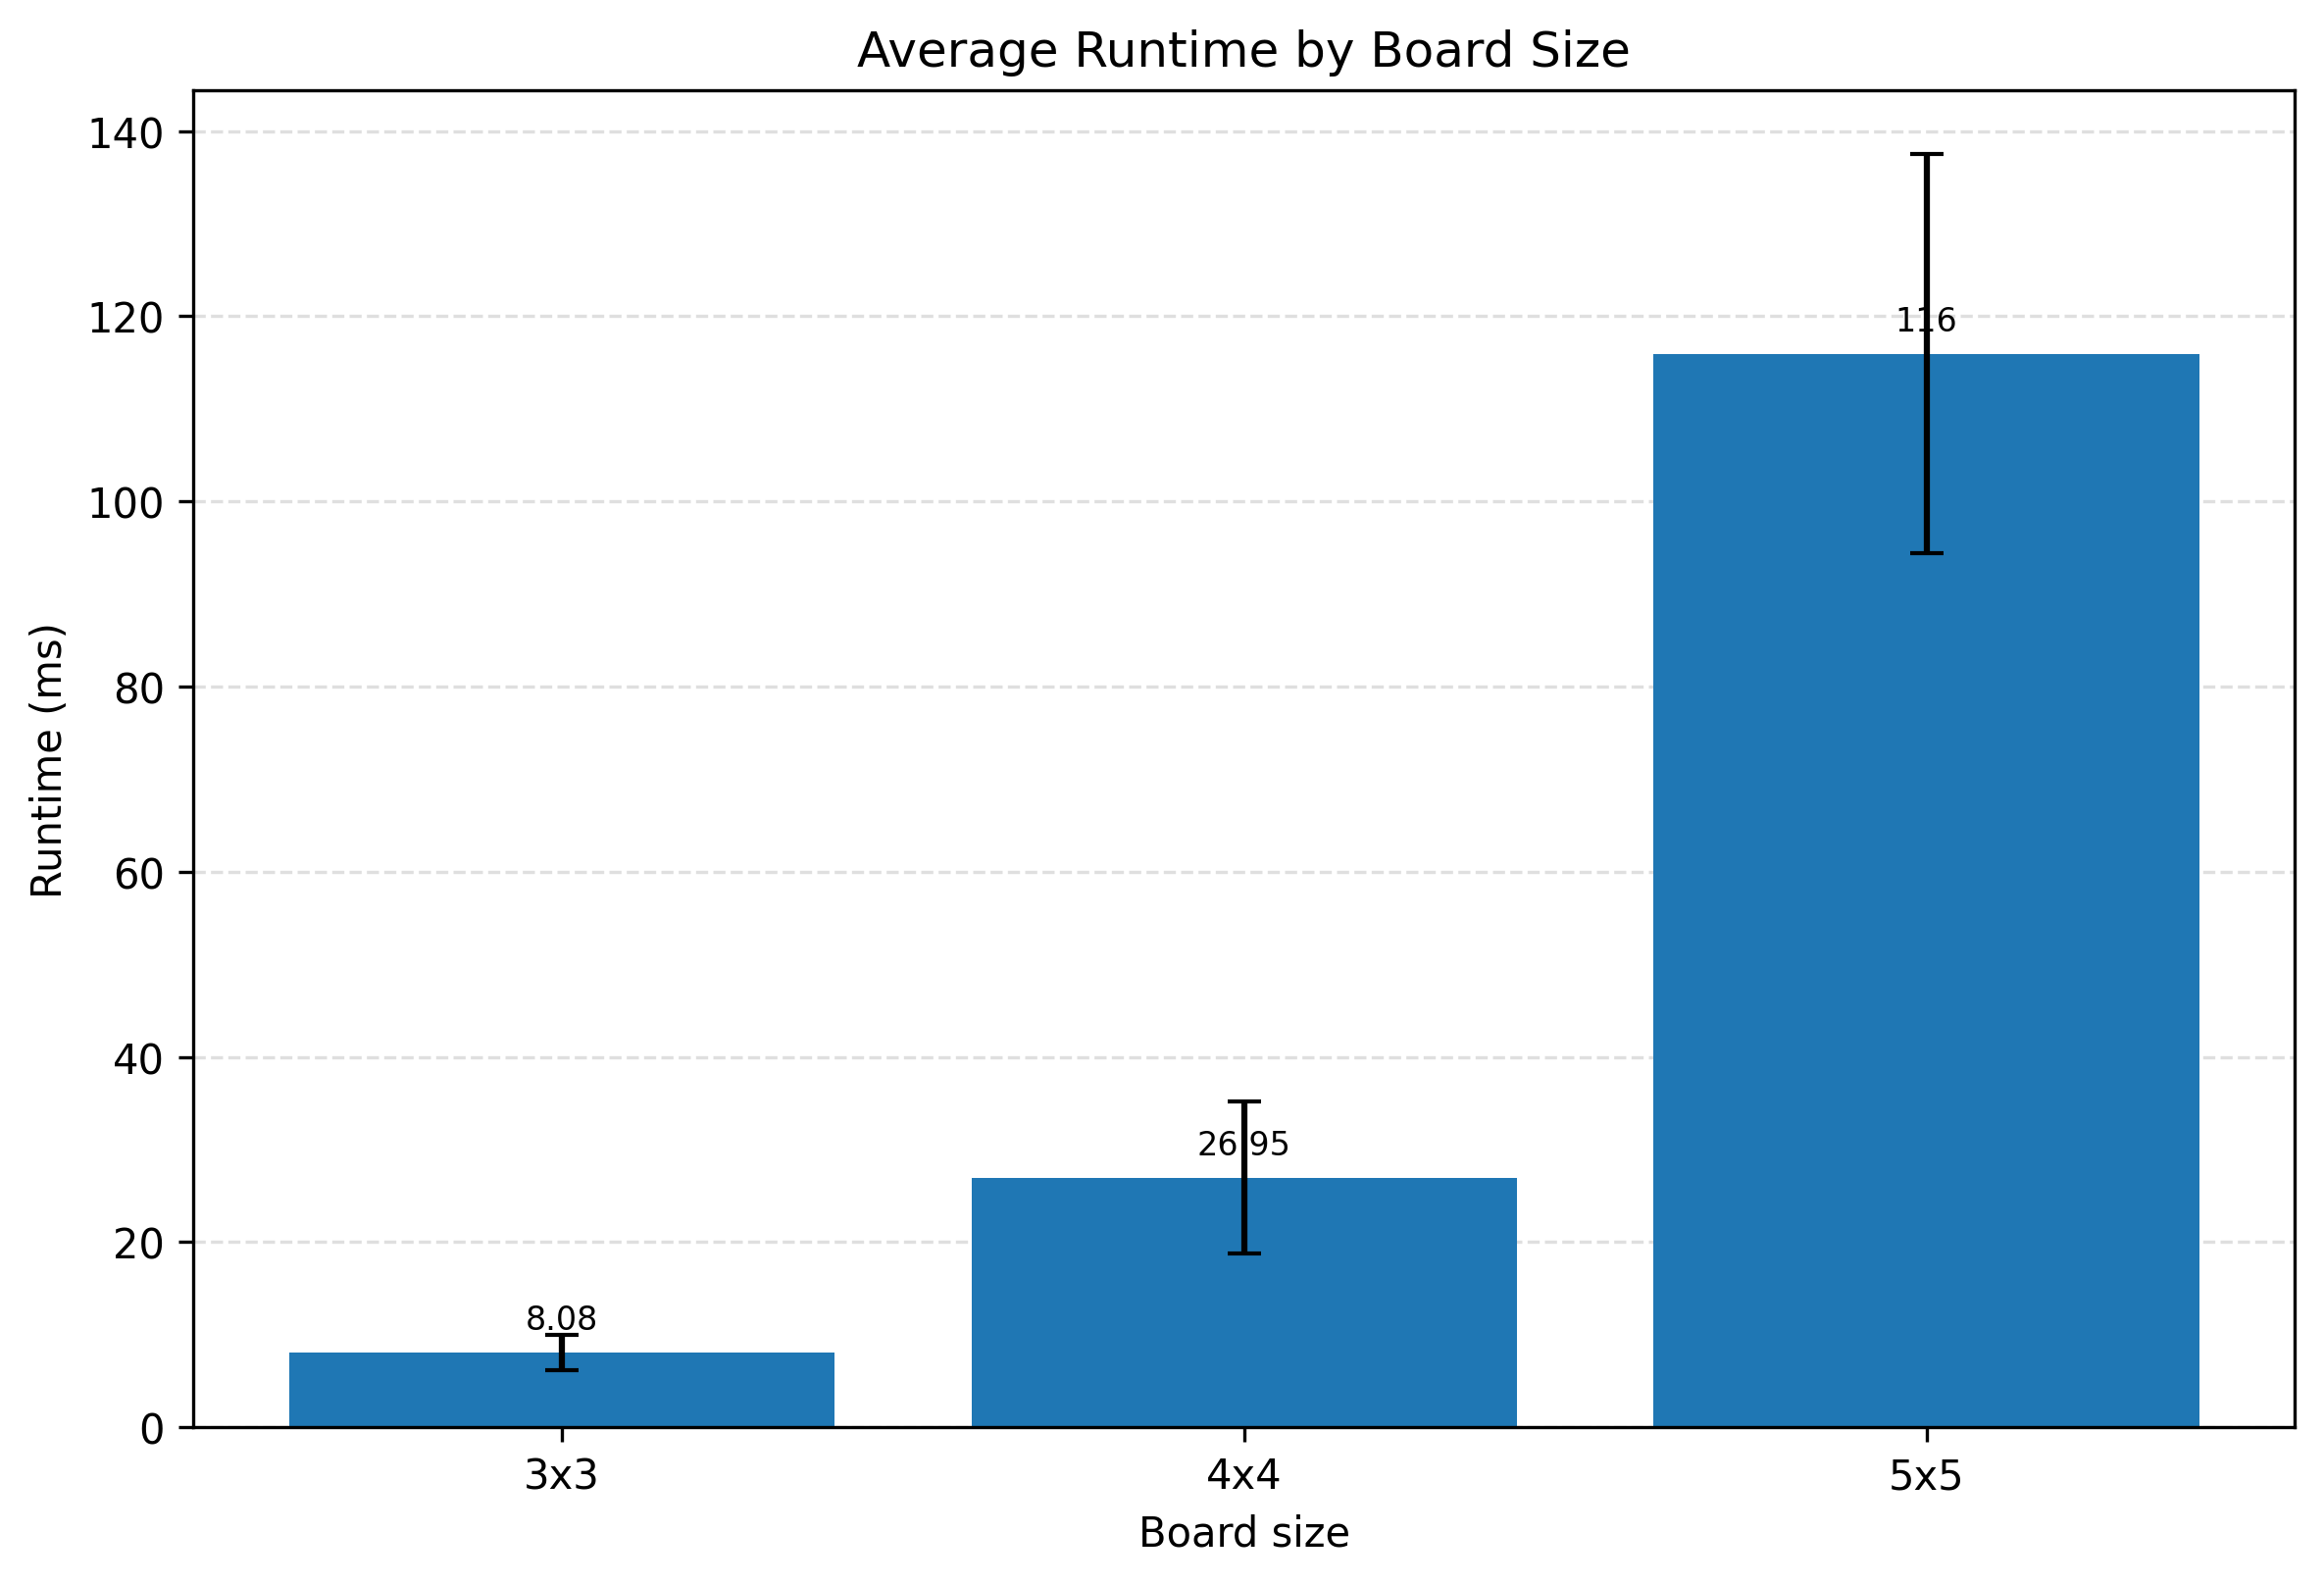
\includegraphics[width=0.88\linewidth]{runtime_by_size.png}
\caption{Runtime trung bình theo kích thước bàn cờ.}
\end{figure}
\begin{figure}[htbp]\centering
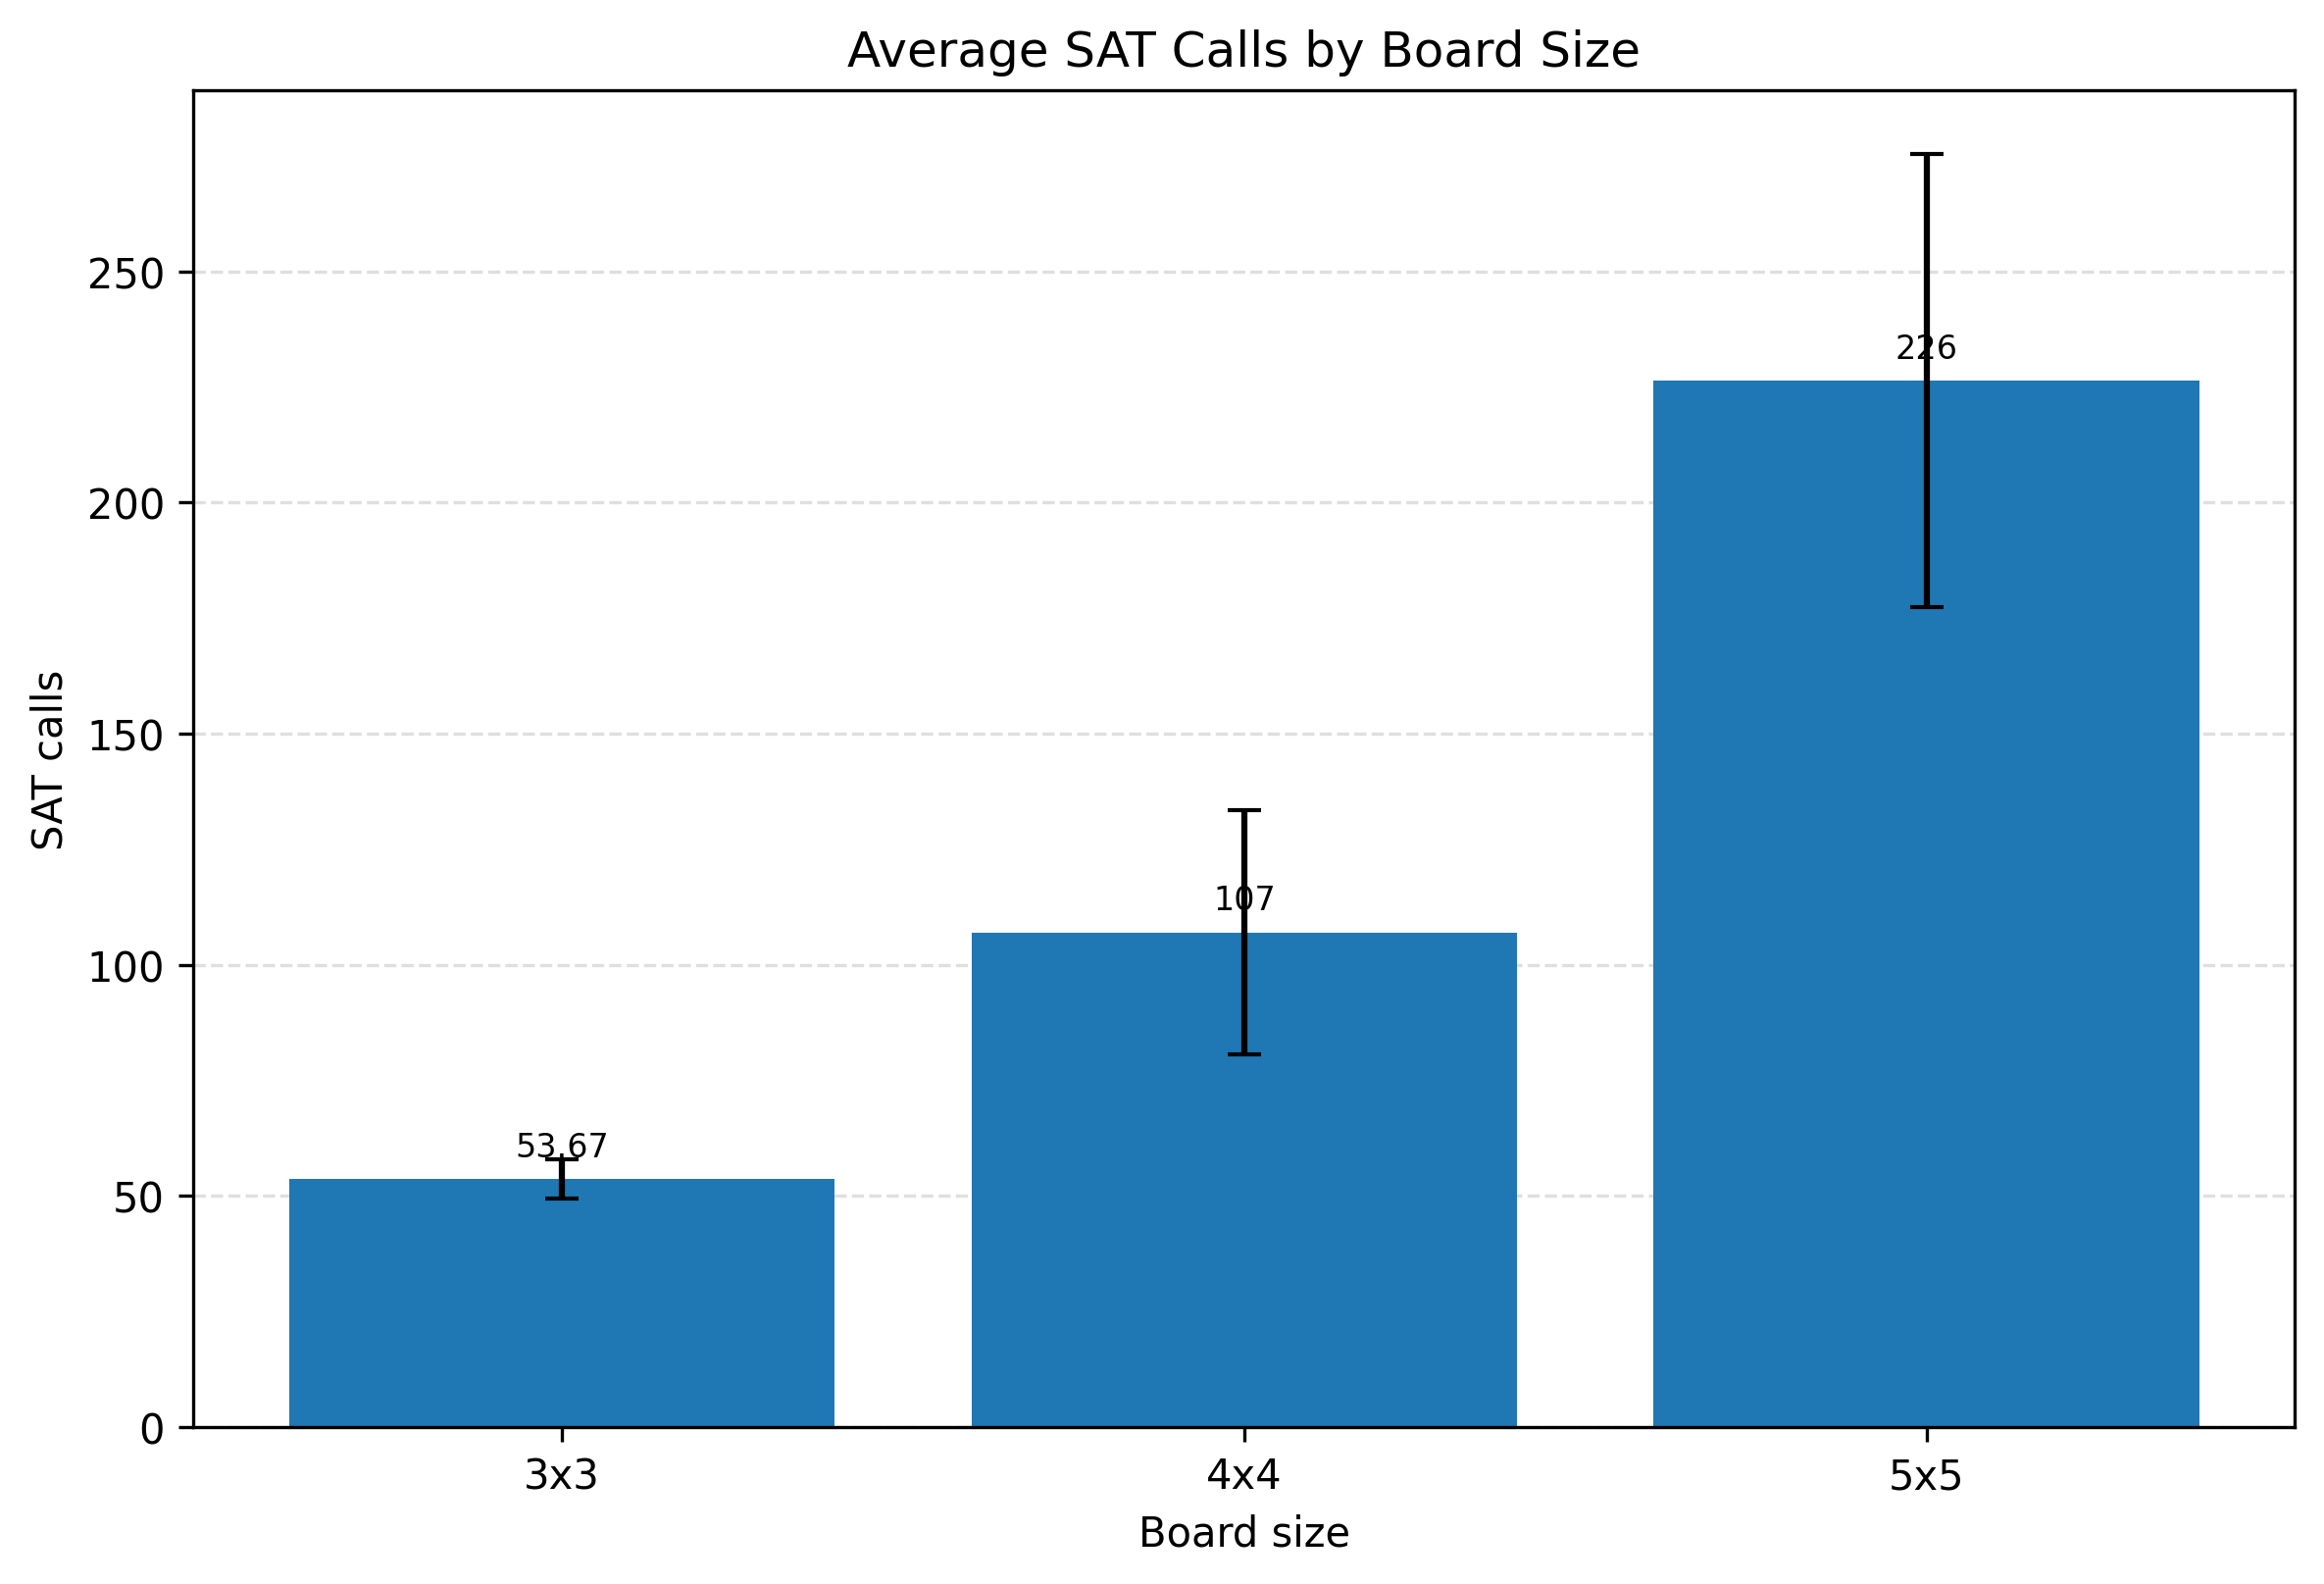
\includegraphics[width=0.88\linewidth]{sat_calls_by_size.png}
\caption{Số lần gọi SAT trung bình theo kích thước.}
\end{figure}
\begin{figure}[htbp]\centering
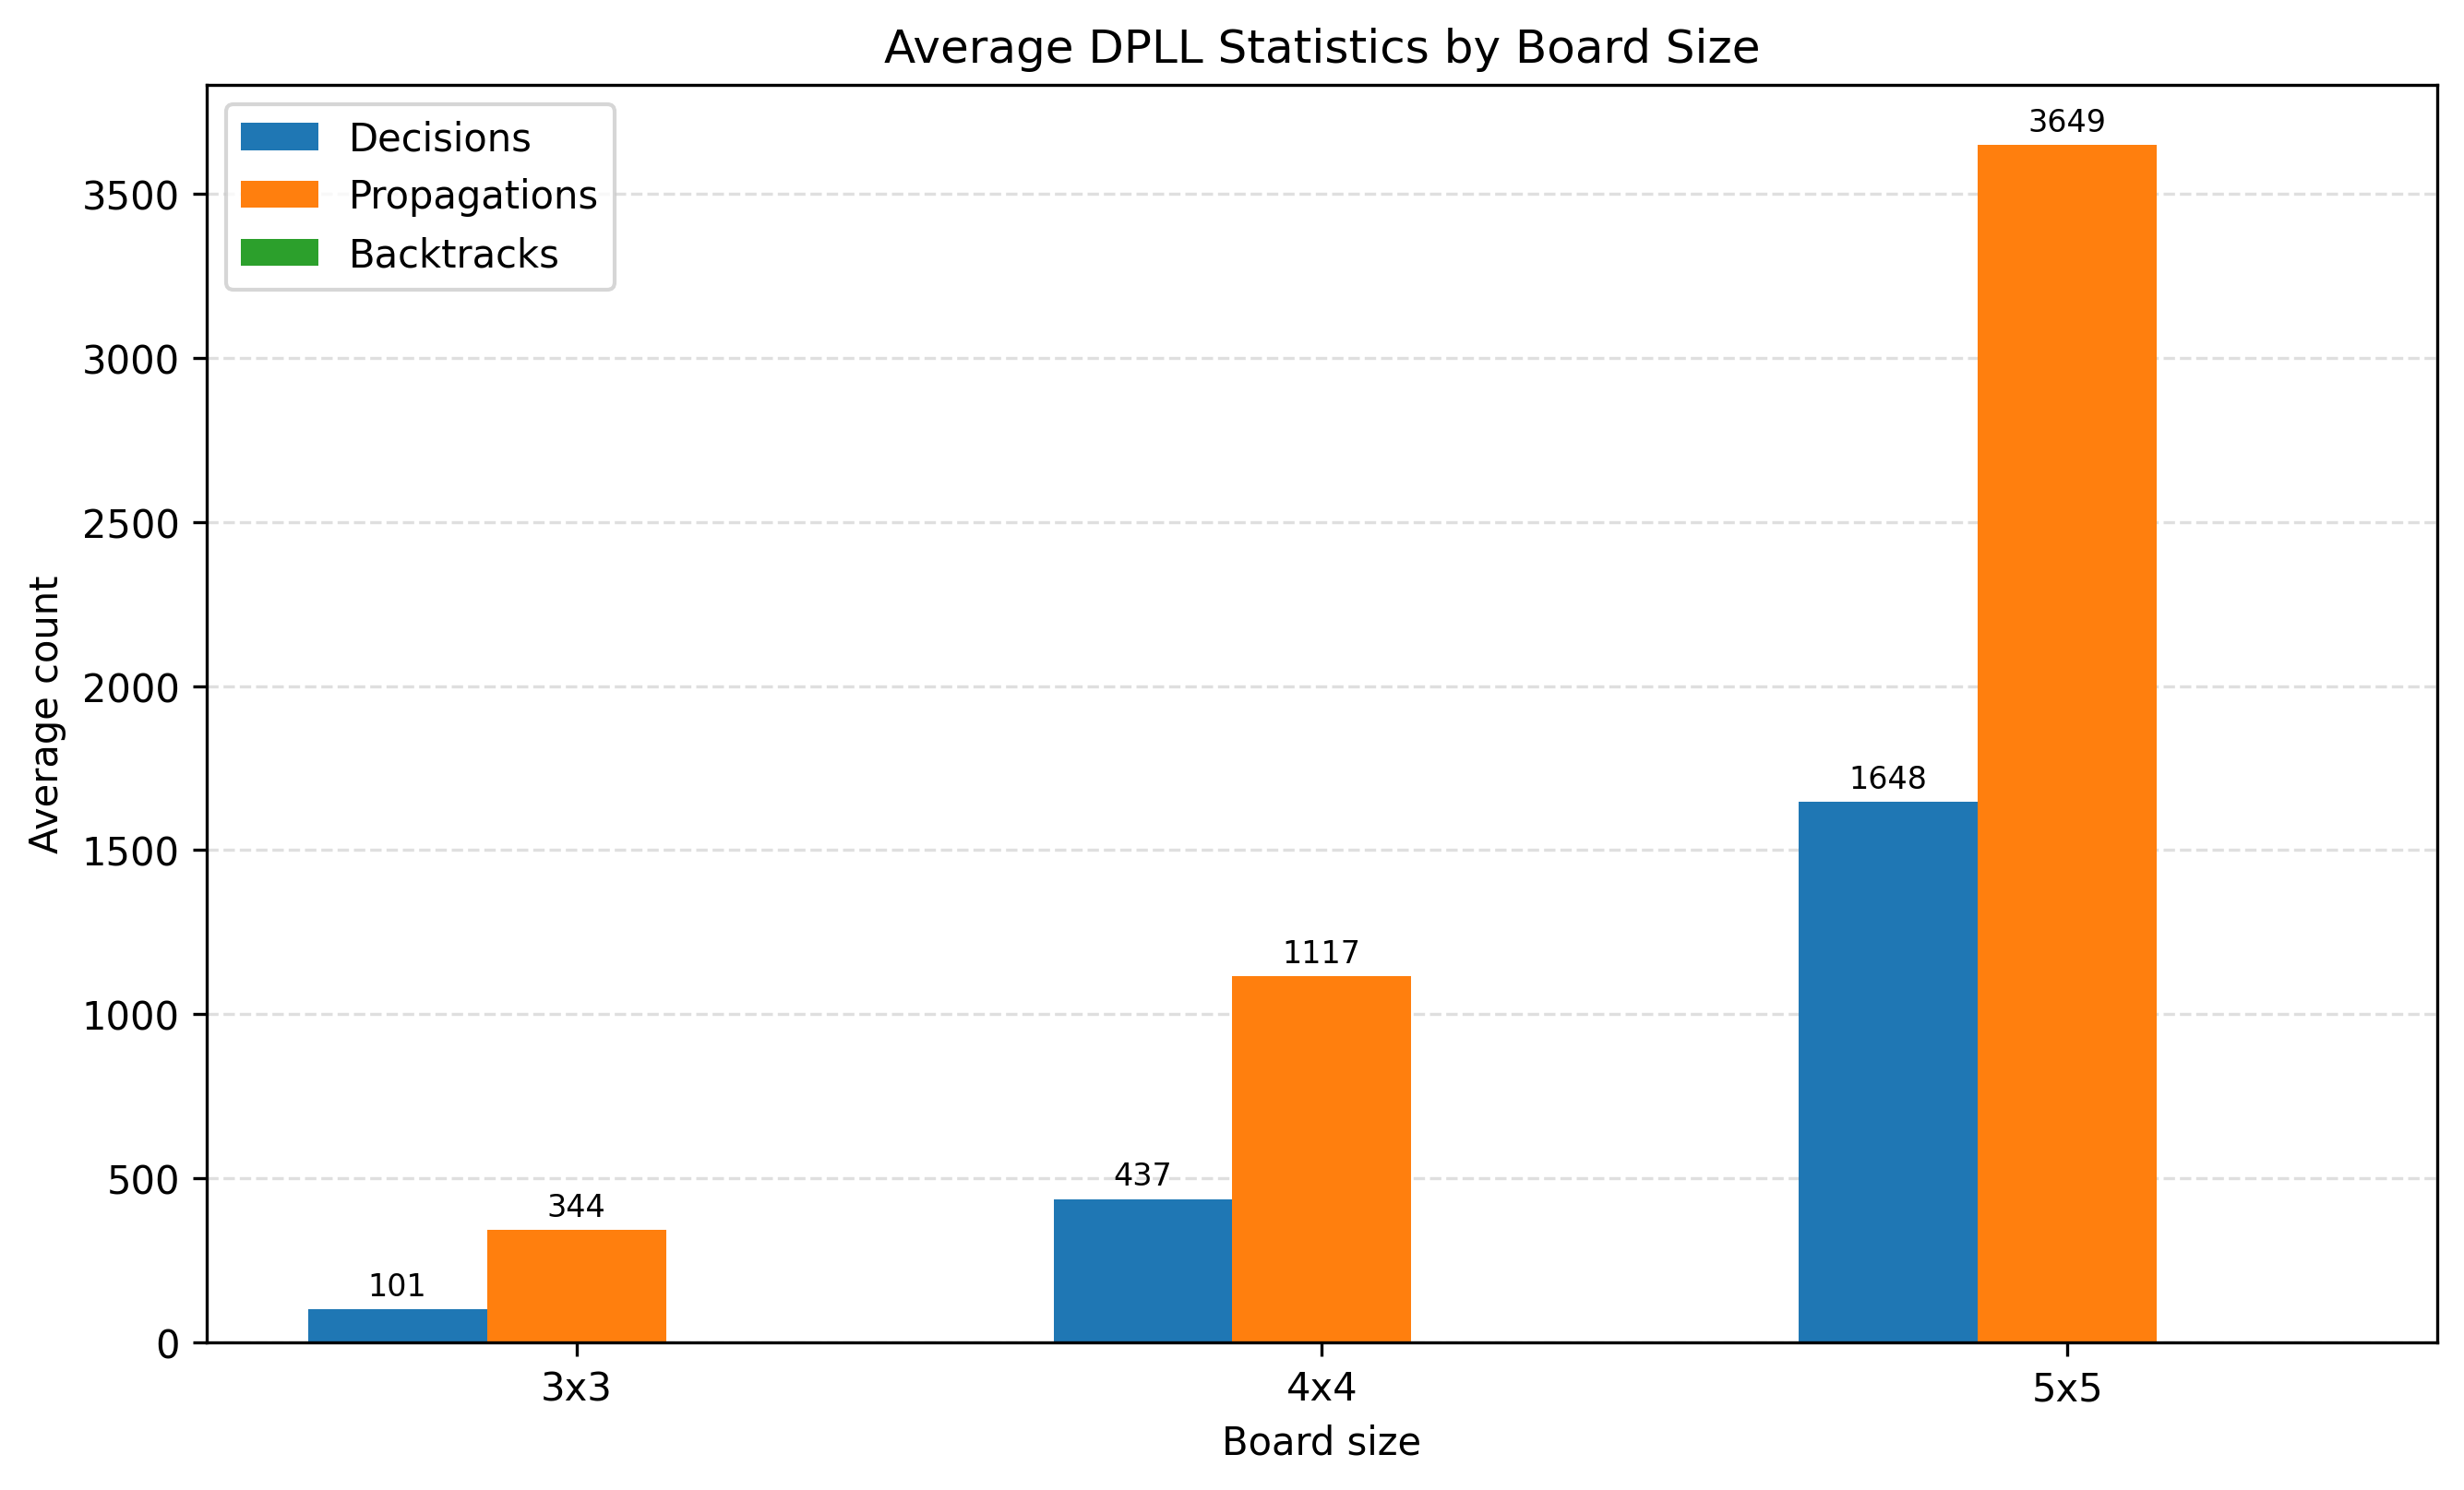
\includegraphics[width=0.88\linewidth]{dpll_statistics_by_size.png}
\caption{Các thống kê DPLL theo kích thước bàn cờ.}
\end{figure}
\subsection{Kết quả theo từng màn chơi}
\begin{figure}[htbp]\centering
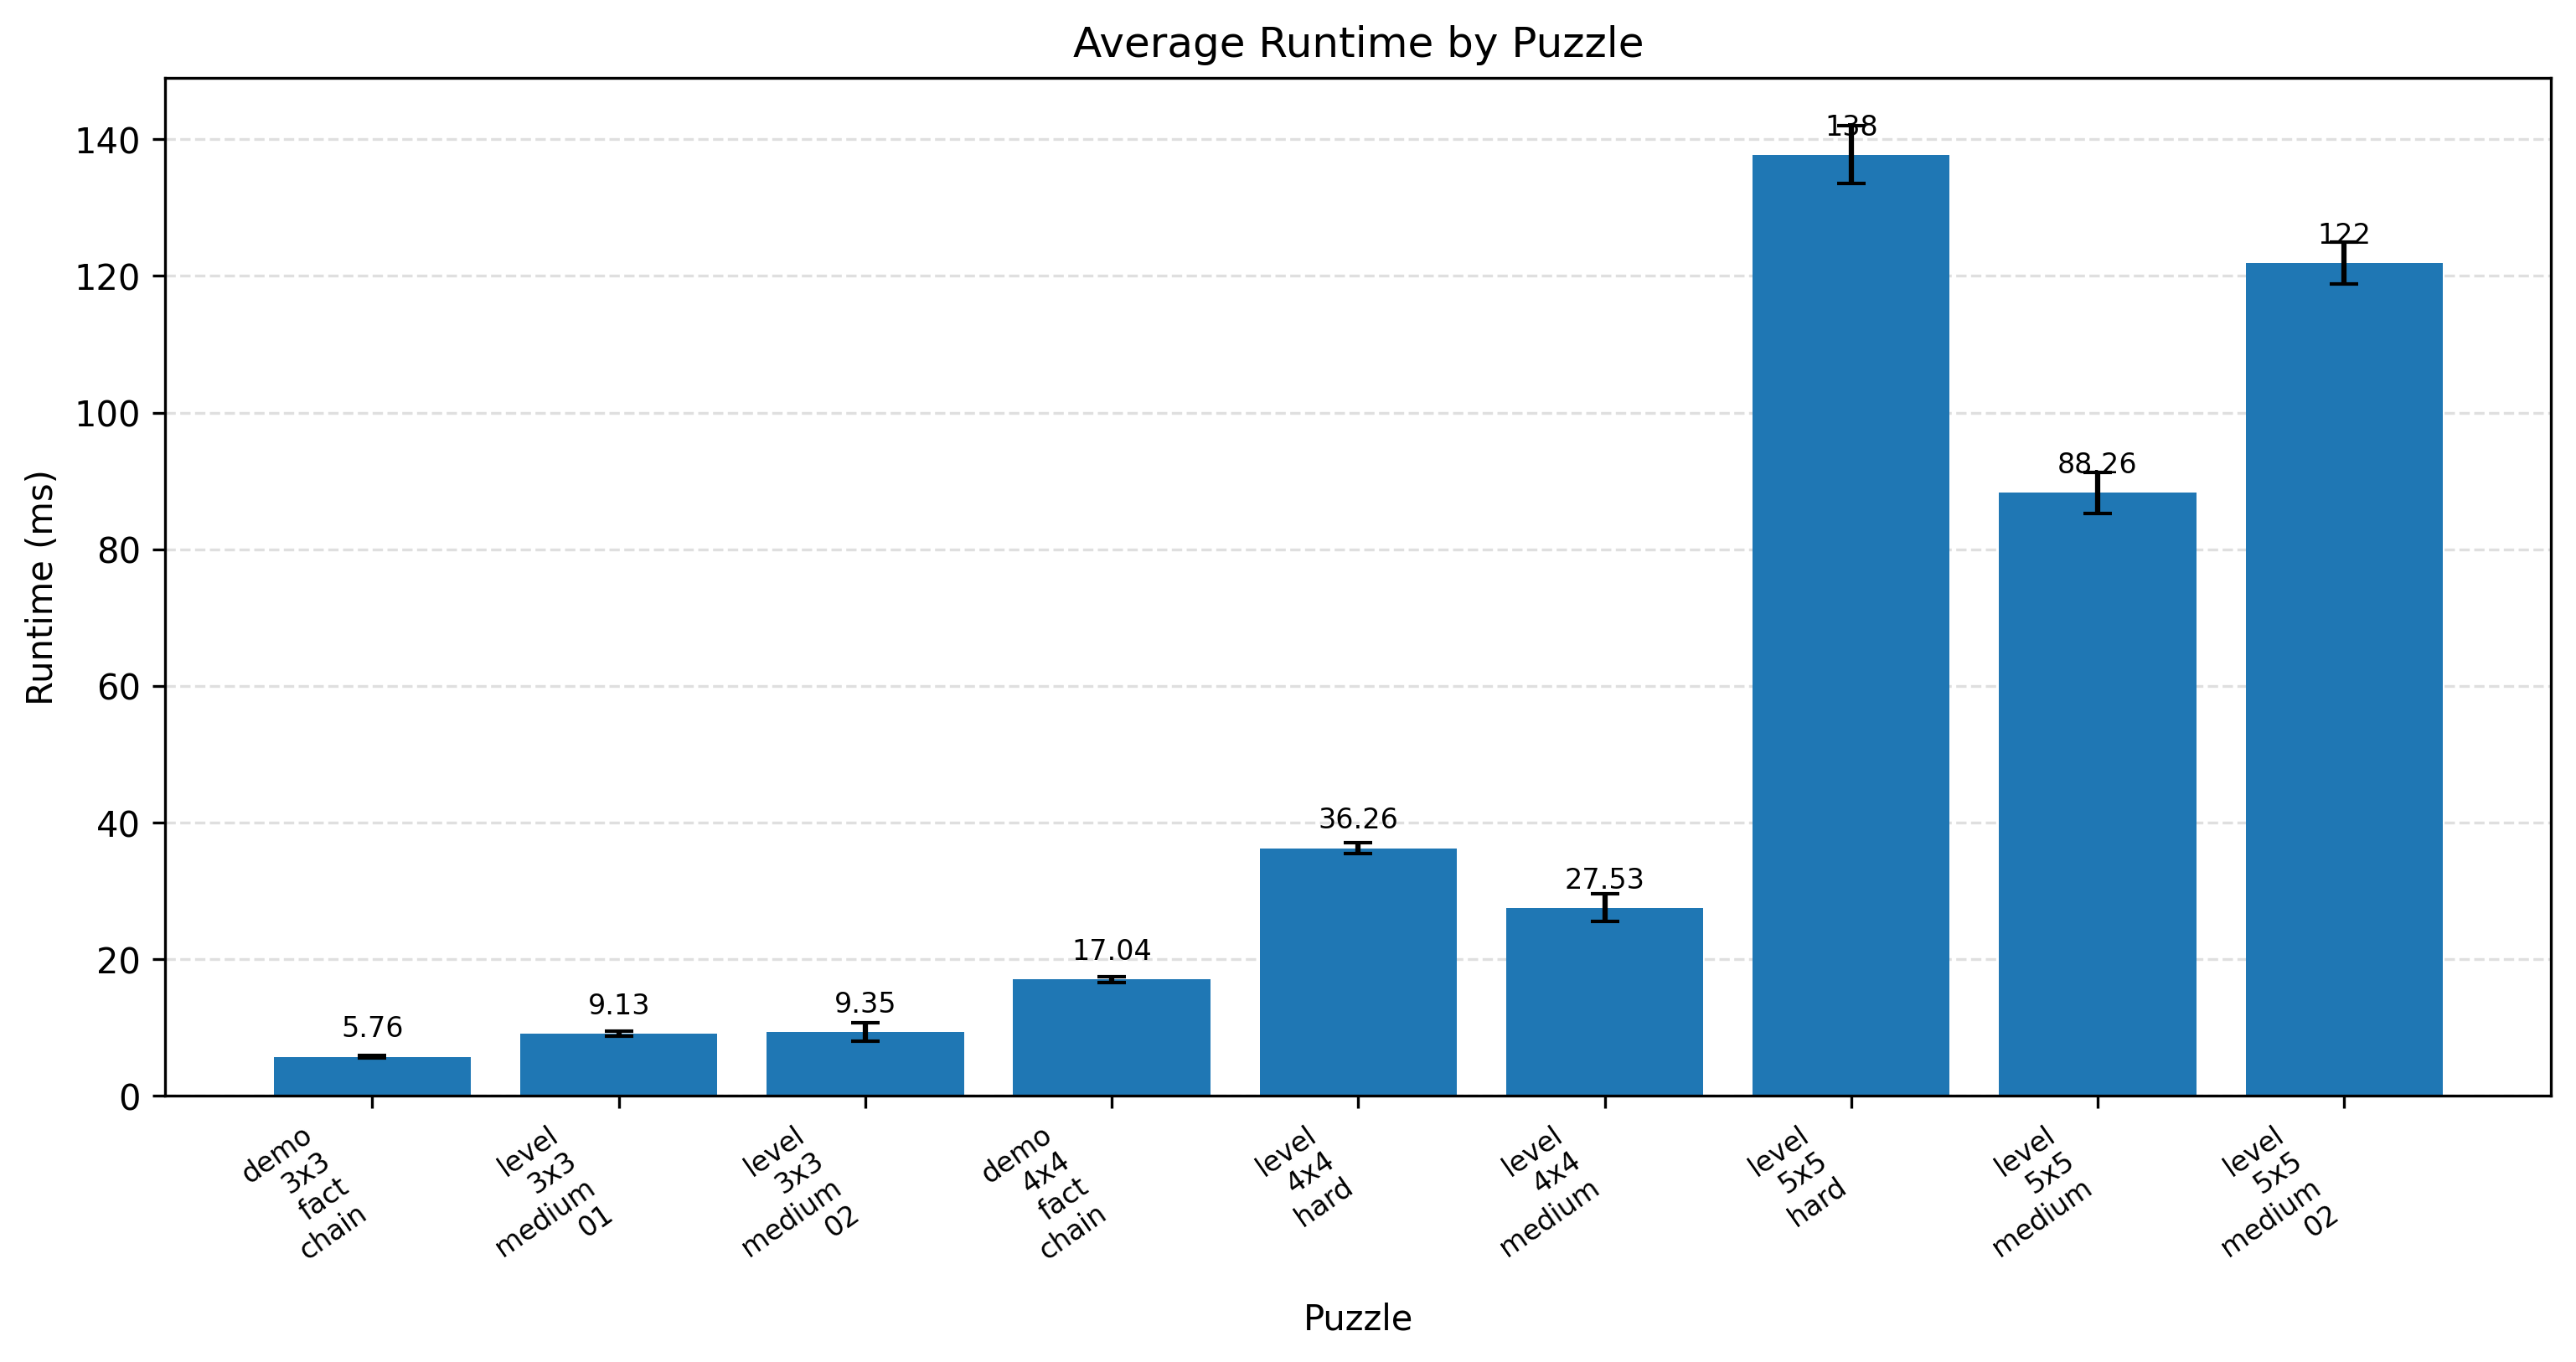
\includegraphics[width=\linewidth]{runtime_by_puzzle.png}
\caption{Runtime trung bình của từng puzzle.}
\end{figure}
\begin{figure}[htbp]\centering
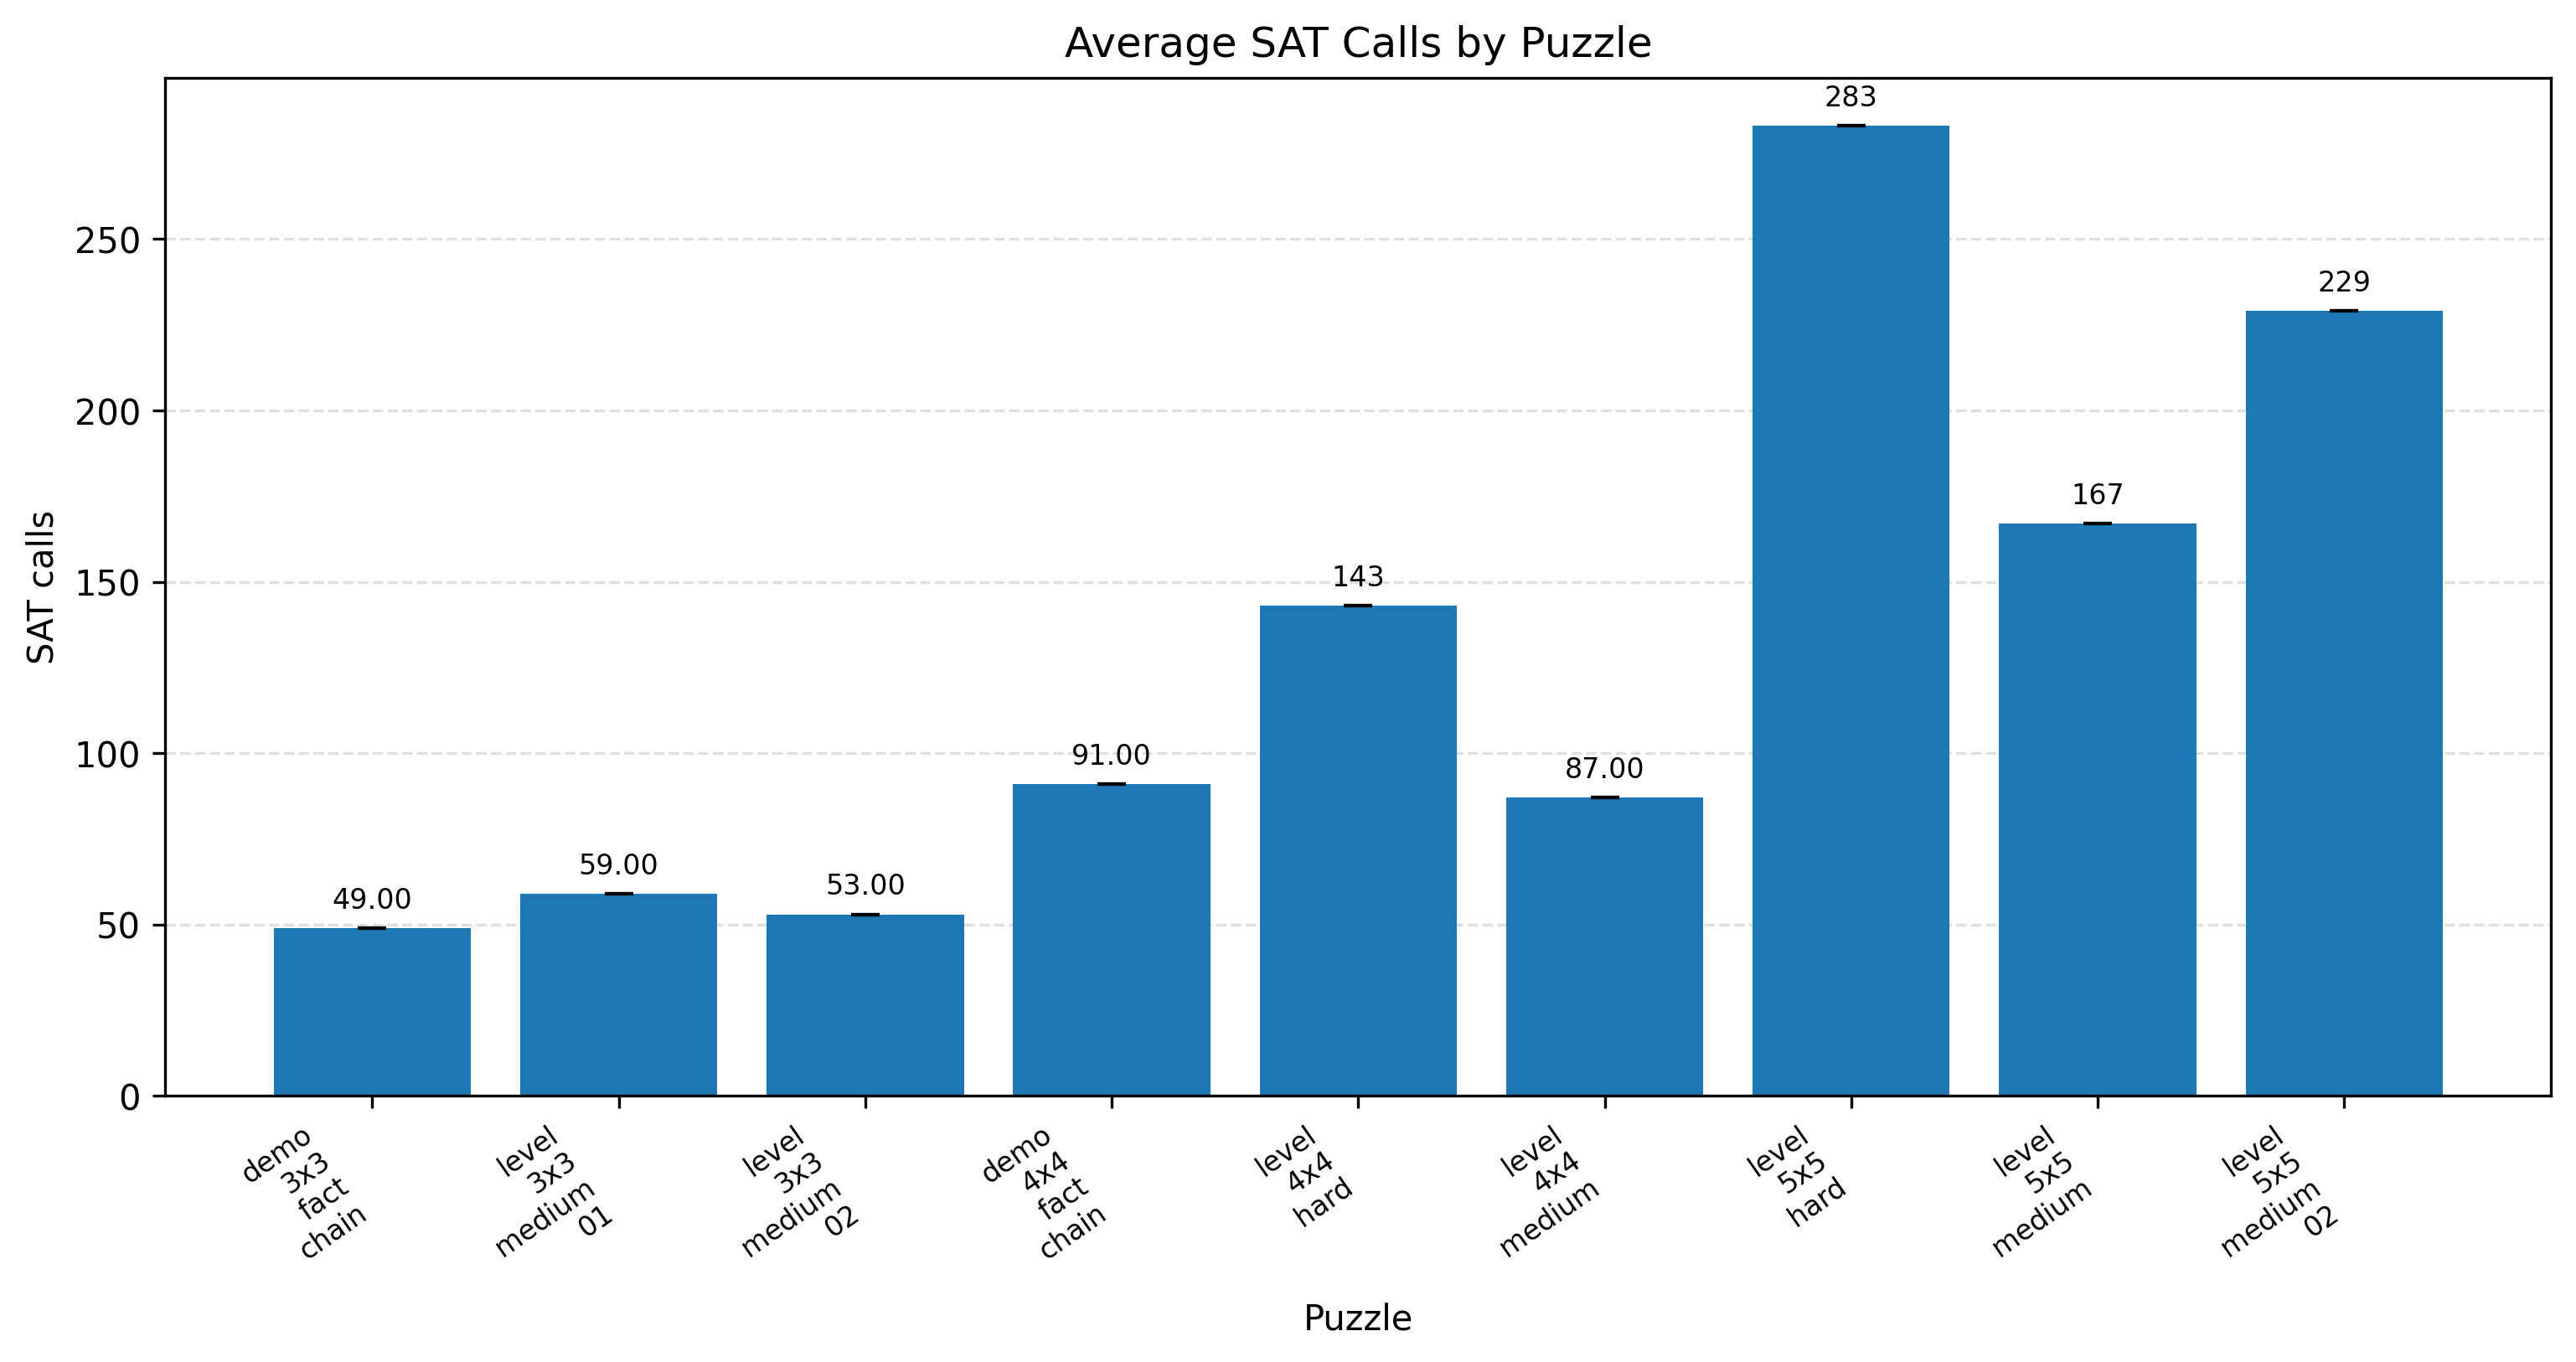
\includegraphics[width=\linewidth]{sat_calls_by_puzzle.png}
\caption{Số lần gọi SAT của từng puzzle.}
\end{figure}
\begin{figure}[htbp]\centering
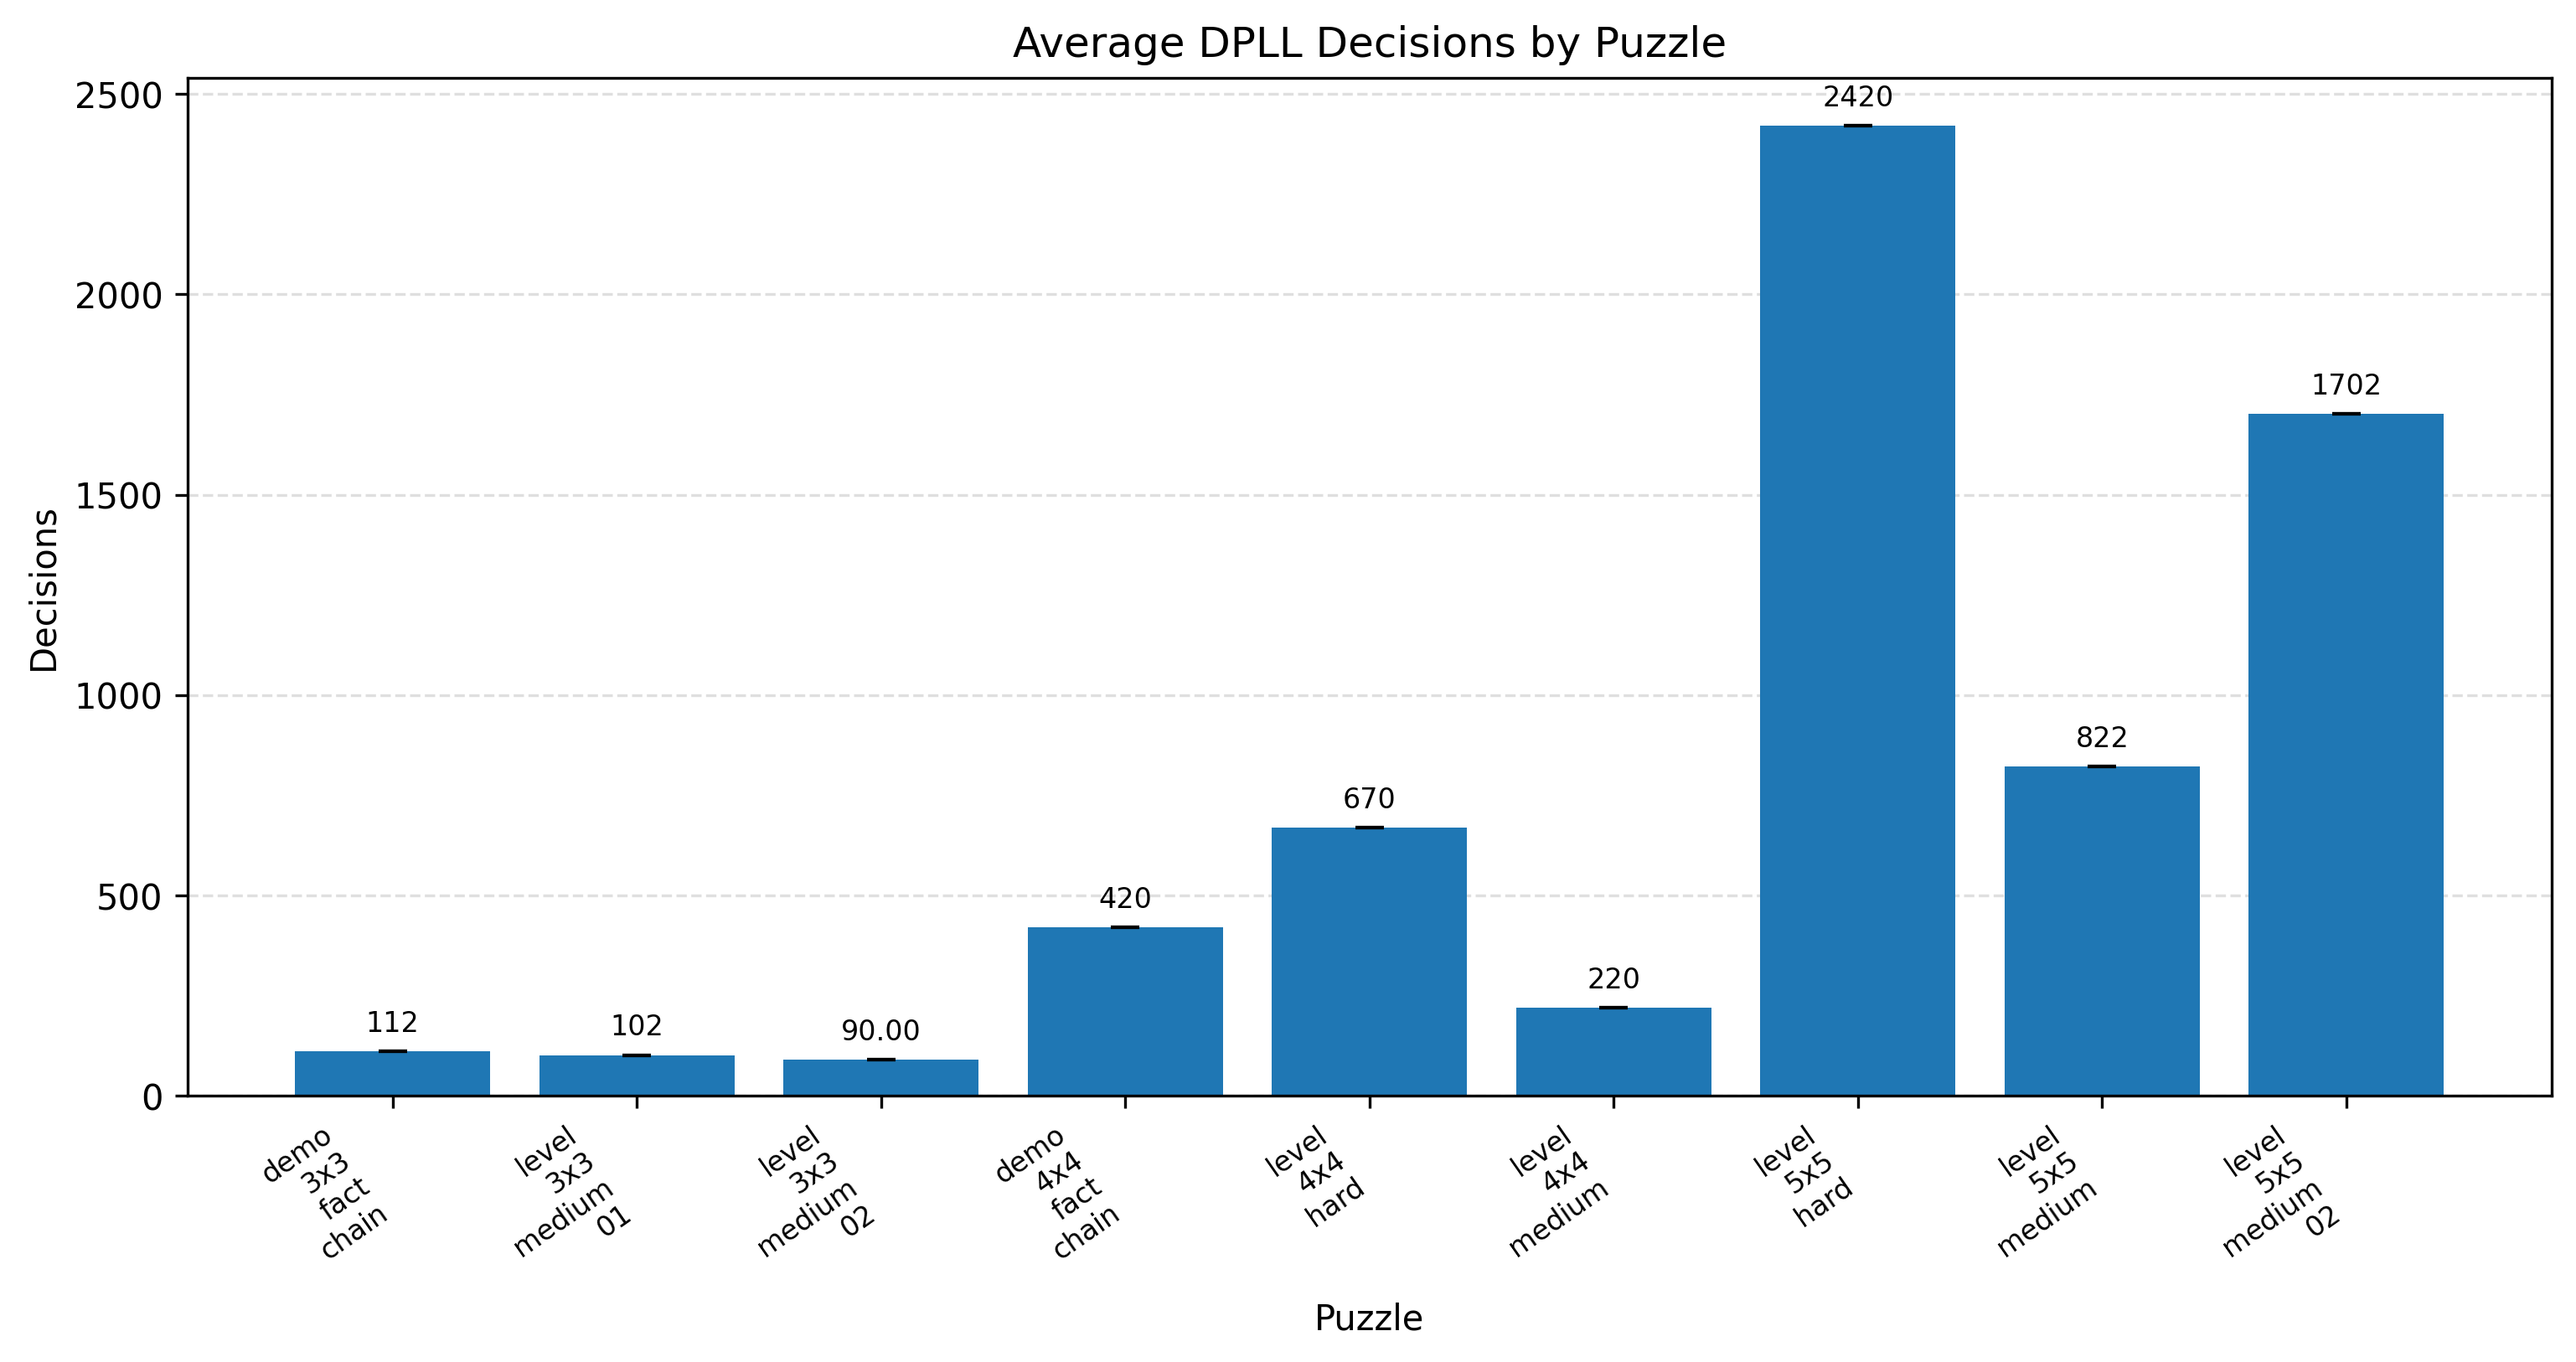
\includegraphics[width=\linewidth]{decisions_by_puzzle.png}
\caption{Số decisions của từng puzzle.}
\end{figure}
\begin{figure}[htbp]\centering
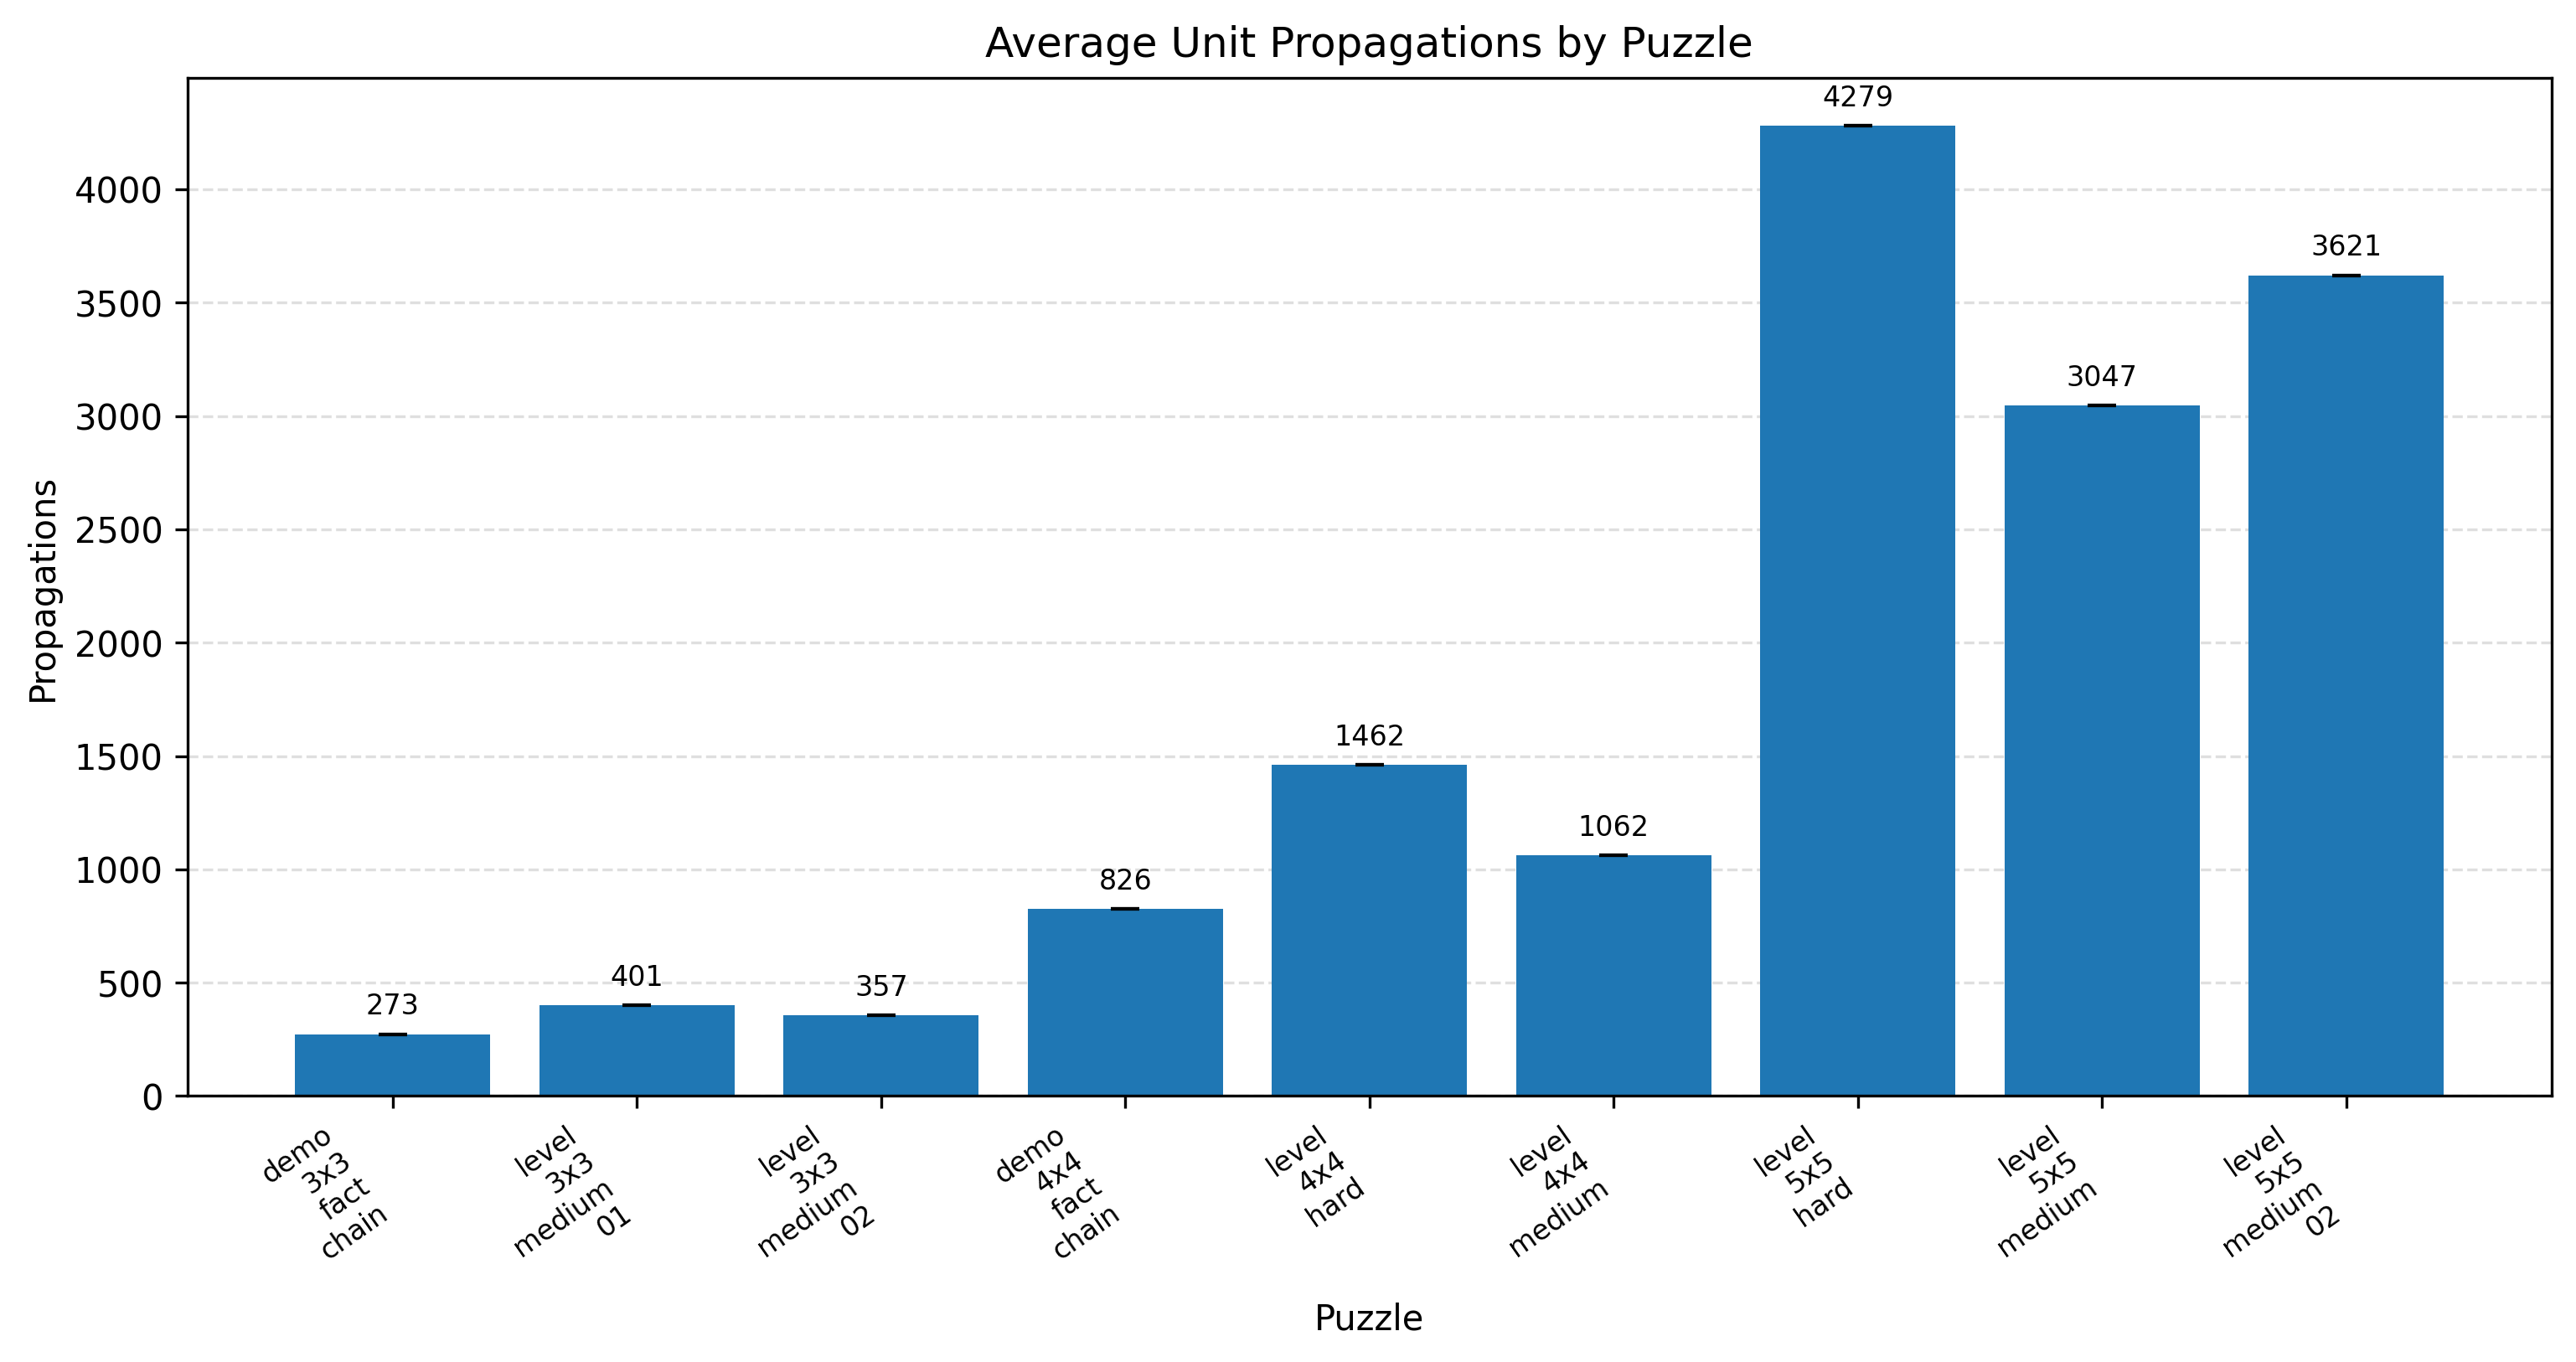
\includegraphics[width=\linewidth]{propagations_by_puzzle.png}
\caption{Số propagations của từng puzzle.}
\end{figure}
\begin{figure}[htbp]\centering
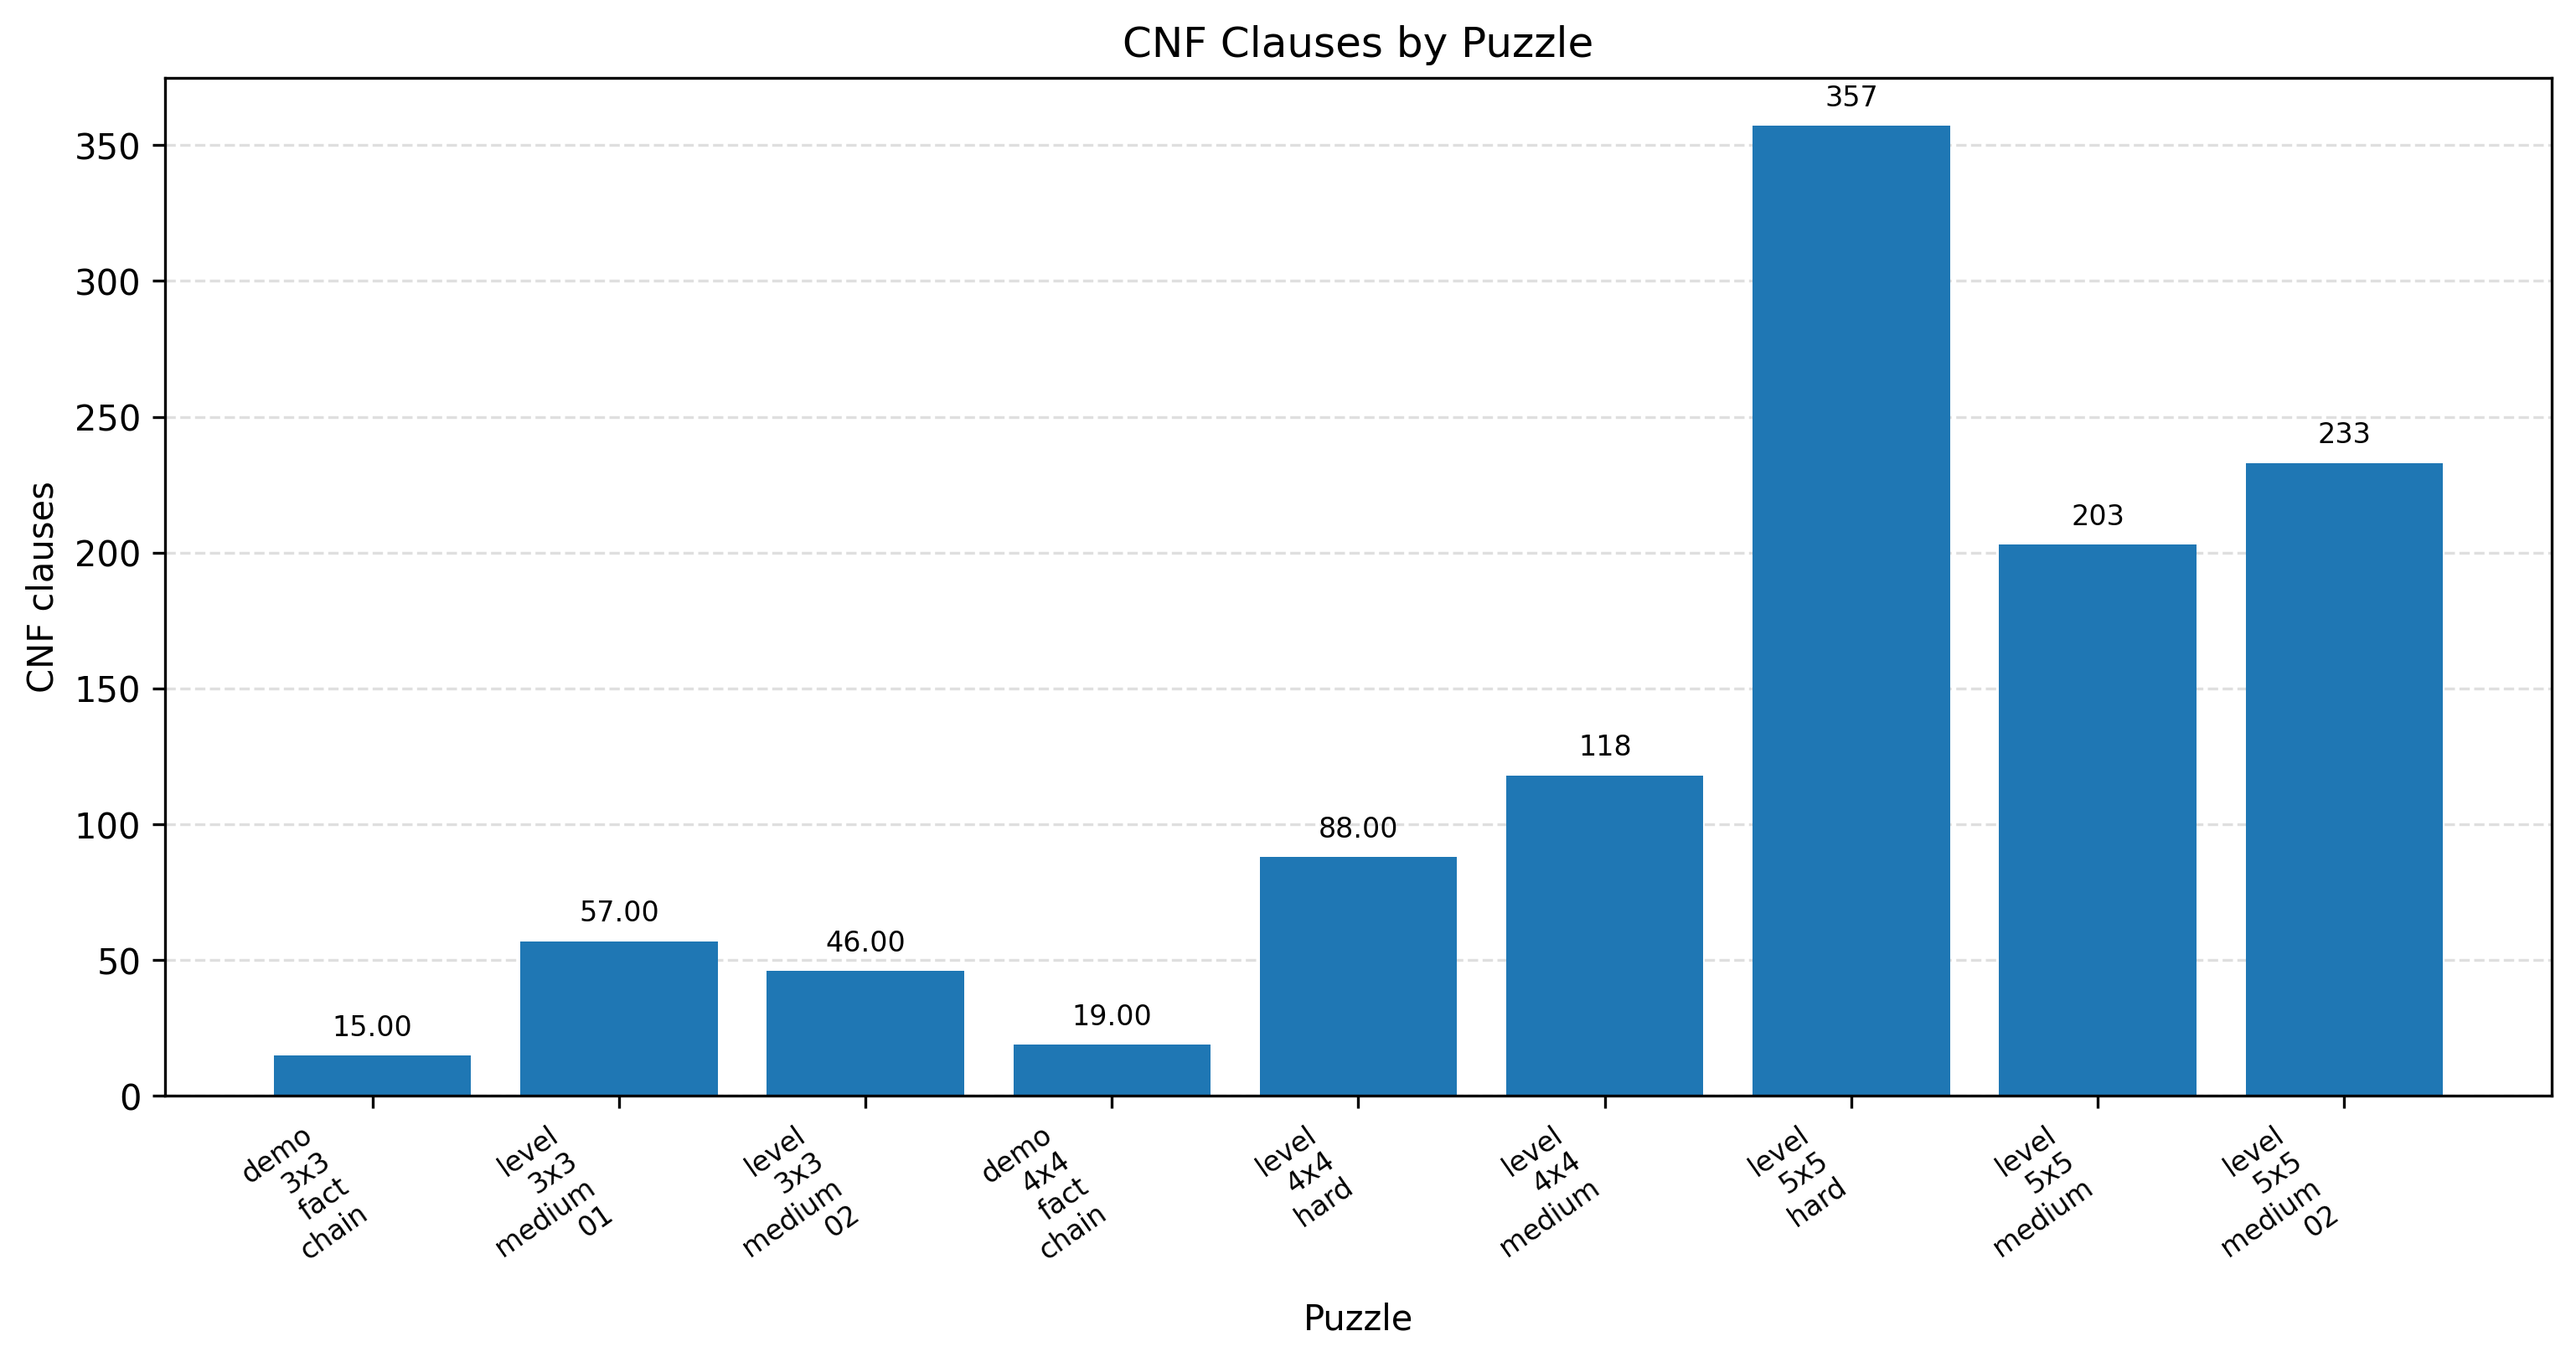
\includegraphics[width=\linewidth]{cnf_clauses_by_puzzle.png}
\caption{Số CNF clauses của từng puzzle.}
\end{figure}
\subsection{Phân tích kết quả}
% Phân tích số liệu từ experiment_size_summary.csv và experiment_summary.csv.
% Không suy rộng ngoài 9 puzzle/45 lượt chạy.
\subsection{Trường hợp đặc biệt và hạn chế}
% Báo cáo demo_4x4 MULTIPLE nhưng SOLVED(5/5) đúng thực tế hiện tại.
% Nêu rõ đây là tính duy nhất khác với khả năng giải tuần tự.
% Cập nhật lại nếu nhóm thay puzzle và chạy lại thí nghiệm.

\clearpage
\section{Kết luận và hướng phát triển}
\subsection{Kết quả đạt được}
Đồ án đã tích hợp trò chơi suy luận trên lưới với bộ mã hóa CNF, thuật
toán DPLL và Logic Agent. Người chơi và tác tử dùng cùng quy tắc mở thẻ:
kết luận phải suy ra được từ manh mối và trạng thái đã công bố tại lượt
đó. Giao diện hỗ trợ chơi thủ công, gợi ý và giải tự động. Bộ kiểm định
xác nhận cả tính duy nhất của nghiệm khi dùng toàn bộ manh mối lẫn khả
năng mở thẻ tuần tự theo luật chơi.

Trong bộ dữ liệu thực nghiệm đã lưu, cả chín màn đều có nghiệm duy nhất
và Agent hoàn tất cả 45 lượt giải. Thời gian giải trung bình theo kích
thước $3\times3$, $4\times4$ và $5\times5$ lần lượt là 9,12 ms, 28,23 ms
và 115,78 ms. Các phép đo này mô tả bộ màn và cấu hình chạy thực nghiệm.

\subsection{Hạn chế}
Bộ dữ liệu có ba màn cho mỗi kích thước và không ghi nhận lần quay lui
nào trong các lượt giải. Do đó, số liệu thời gian hiện tại chưa thể hiện
chi phí của DPLL trên các màn cần tìm kiếm qua nhiều nhánh. Mã hóa tổ
hợp trực tiếp có thể sinh nhiều mệnh đề khi vùng đếm lớn. Agent cũng
xây lại CNF ở mỗi lần gọi và giải độc lập các truy vấn SAT, kể cả khi
các truy vấn dùng chung phần lớn mệnh đề. Nhật ký lưu các manh mối đang
công khai và kết quả truy vấn, nên người chơi chưa có lời giải thích
chỉ ra tập tiền đề nhỏ đủ để chứng minh một kết luận.

\subsection{Hướng phát triển}
Có thể mở rộng bộ màn bằng các trường hợp buộc DPLL quay lui và các
màn có nghiệm duy nhất nhưng bị kẹt ở trạng thái công khai. Với vùng
đếm lớn, có thể so sánh mã hóa tổ hợp với bộ đếm tuần tự theo số mệnh
đề, số biến phụ và thời gian giải. Một hướng khác là tái sử dụng phần
CNF chung giữa các lượt và dùng giả định tạm trong bộ giải SAT tăng
dần. Khi cải tiến gợi ý, có thể tìm một tập manh mối đủ để chứng minh
nước đi và diễn giải tập đó bằng câu mô tả phù hợp với giao diện.


\clearpage
\phantomsection
\addcontentsline{toc}{section}{Tài liệu tham khảo}
\begin{thebibliography}{9}
\bibitem{de} Khoa Công nghệ Thông tin, Trường Đại học Khoa học Tự nhiên, ĐHQG-HCM. \textit{CSC14003 Introduction to Artificial Intelligence, Project 2: Griductive Solver} [Đề bài học phần].
\bibitem{dpll} M. Davis, G. Logemann, and D. Loveland. \textit{A Machine Program for Theorem-Proving}. Communications of the ACM, 5(7), 1962, pp. 394--397.
\bibitem{aima} S. Russell and P. Norvig. \textit{Artificial Intelligence: A Modern Approach}. 4th edition, Pearson, 2021.
\bibitem{griductive} Griductive. \textit{How to Play}. \url{https://griductive.com/}.
\end{thebibliography}

\appendix
\section{Mã nguồn và video demo}
\begin{itemize}
    \item Mã nguồn Griductive Solver trên GitHub\par
    \url{https://github.com/hohuunghiem/Fundamentals-of-Artificial-Intelligence-Griductive-Solver}
    \item Video demo Griductive Solver trên Google Drive\par
    \url{https://drive.google.com/file/d/1NBbvhKspHTGH47xaYmq9ht4gE7EEVJkj/view}
\end{itemize}

\section{Hướng dẫn cài đặt và chạy chương trình}
\begin{lstlisting}[language=bash]
# Create and activate the environment
conda create -n lab2 python=3.10 pip -y
conda activate lab2

# Install dependencies
cd Source
pip install -r requirements.txt

# Run the game
python main.py

# Run tests
python -m unittest discover -s tests -v
\end{lstlisting}

Chạy thực nghiệm trên Linux (ví dụ Ubuntu) vì chương trình dùng
\texttt{SIGALRM} để giới hạn thời gian từng lượt. Trên Windows có
thể dùng WSL với Ubuntu. Chạy các lệnh dưới đây từ \texttt{Source/}
sau khi cài thư viện trong môi trường Linux.
\begin{lstlisting}[language=bash]
# Run repeated experiments
python -m experiments.run_experiments

# Generate charts
python -m experiments.plot_results
\end{lstlisting}

\clearpage
\section{Phân công công việc}
\begin{table}[H]\centering
\caption{Phân công công việc của nhóm}
\begin{tabularx}{\linewidth}{|p{0.27\linewidth}|Y|}
\hline
Thành viên & Công việc phụ trách\\\hline
Chu Bảo Minh & Core Game; điều phối báo cáo; video demo.\\\hline
Võ Trúc Quỳnh & CNF Encoder.\\\hline
Trần Thị Bích Hạnh & DPLL SAT Solver.\\\hline
Huỳnh Thanh Huy & Logic Agent.\\\hline
Hồ Hữu Nghiêm & Validator và Experiments.\\\hline
\end{tabularx}
\end{table}

\section{Khai báo sử dụng công cụ AI}
OpenAI Codex được dùng để hỗ trợ đọc mã nguồn, đối chiếu nội dung với
kiểm thử và số liệu đã lưu, đồng thời hỗ trợ soạn thảo và chỉnh sửa
các mục Tổng quan, Mô hình hóa bài toán, Logic Agent, Cài đặt và giao
diện, Thực nghiệm và đánh giá, Kết luận và Phụ lục của báo cáo LaTeX.
Các số liệu trình bày trong báo cáo lấy từ tệp kết quả của chương trình
thực nghiệm. Kết quả kiểm thử được lấy từ lần chạy bộ kiểm thử Python.

\end{document}
